\documentclass[journal]{IEEEtran}
\usepackage{gvv-book}
\usepackage{gvv}
%\usepackage{styles/front}
%\usepackage{Wiley-AuthoringTemplate}
%\usepackage[sectionbib,authoryear]{natbib}% for name-date citation comment the below line
%\usepackage[sectionbib,numbers]{natbib}% for numbered citation comment the above line

%%********************************************************************%%
%%       How many levels of section head would you like numbered?     %%
%% 0= no section numbers, 1= section, 2= section, 3= subsection %%
\setcounter{secnumdepth}{3}
%%********************************************************************%%
%%**********************************************************************%%
%%     How many levels of section head would you like to appear in the  %%
%%				Table of Contents?			%%
%% 0= chapter, 1= section, 2= section, 3= subsection titles.	%%
\setcounter{tocdepth}{2}
%%**********************************************************************%%

%\includeonly{ch01}
\makeindex

\begin{document}
\bibliographystyle{IEEEtran}
\onecolumn


\title{
	\begin{flushleft}
	MATRICES \\ In Geometry
	\\
\rule{0.4\columnwidth}{0.4pt}
\end{flushleft}
}
\author{
\vspace{7cm}
	\begin{flushleft}
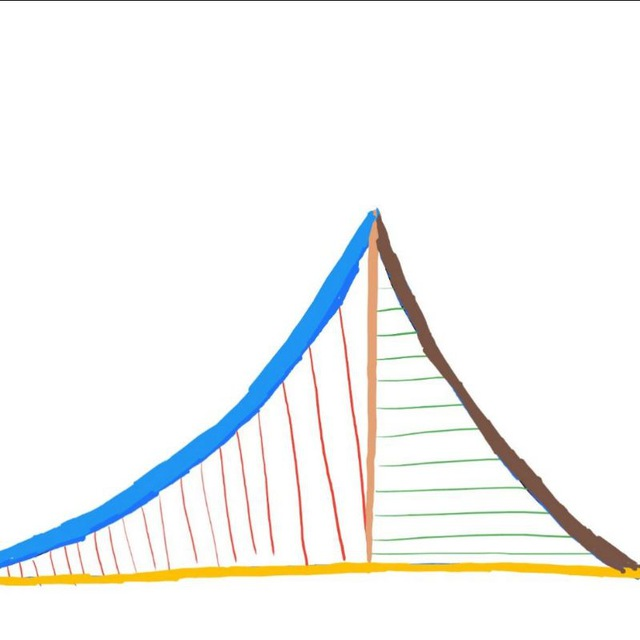
\includegraphics[width=0.2\columnwidth]{figs/logo.jpg}
\\
		{	\huge G. V. V. Sharma}
		\\
\vspace{1cm}
https://creativecommons.org/licenses/by-sa/3.0/
\\
and
\\
https://www.gnu.org/licenses/fdl-1.3.en.html
	\end{flushleft}
%\IEEEpubid{\makebox[\columnwidth]{978-1-7281-5966-1/20/\$31.00 ©2020 IEEE \hfill} \hspace{\columnsep}\makebox[\columnwidth]{ }}
}
\maketitle

\newpage


\tableofcontents

\newpage
\twocolumn

%\section{Triangle}
\section{Vectors}
Consider a triangle with vertices
		\begin{align}
			\label{eq:tri-pts}
			\vec{A} = \myvec{1 \\ -1},\,
			\vec{B} = \myvec{-4 \\ 6},\,
			\vec{C} = \myvec{-3 \\ -5}
		\end{align}
\subsection{Sides}
%\renewcommand{\theequation}{\theenumi}
\begin{enumerate}[label=\thesubsection.\arabic*.,ref=\thesubsection.\theenumi]
\numberwithin{equation}{enumi}
\item The direction vector of $AB$ is defined as
		\begin{align}
			\vec{B}-
			\vec{A}
		\end{align}
Find the direction vectors of $AB, BC$ and $CA$.
\\
\solution 
\begin{enumerate} 
\item  The Direction vector of $AB$ is 
	\begin{align}  \vec{B} - \vec{A} 
		=\myvec{ -4\\ 6 } - \myvec{ 1\\ -1 }
 = \myvec{ -4 - 1\\ 6 - (-1) } = \myvec{ -5\\ 7 }
		\label{eq:geo-dir-vec-ab}
 \end{align}
\item The Direction vector of $BC$ is
	\begin{align} \vec{C} - \vec{B}=\myvec{ -3\\ -5} - \myvec{ -4\\ 6 }
 = \myvec{ -3 - (-4)\\ -5 - 6 } = \myvec{1\\ -11 }
		\label{eq:geo-dir-vec-bc}
  \end{align}
  \item  The Direction vector of $CA$  is
	  \begin{align}  \vec{A} - \vec{C} =\myvec{ 1\\ -1 }-\myvec{ -3\\ -5}
 = \myvec{ 1 - (-3)\\ -1 - (-5) } = \myvec{ 4\\ 4 }
		\label{eq:geo-dir-vec-ca}
  \end{align}
 \end{enumerate}
%	\solution 
\begin{enumerate} 
\item  The Direction vector of $AB$ is 
	\begin{align}  \vec{B} - \vec{A} 
		=\myvec{ -4\\ 6 } - \myvec{ 1\\ -1 }
 = \myvec{ -4 - 1\\ 6 - (-1) } = \myvec{ -5\\ 7 }
		\label{eq:geo-dir-vec-ab}
 \end{align}
\item The Direction vector of $BC$ is
	\begin{align} \vec{C} - \vec{B}=\myvec{ -3\\ -5} - \myvec{ -4\\ 6 }
 = \myvec{ -3 - (-4)\\ -5 - 6 } = \myvec{1\\ -11 }
		\label{eq:geo-dir-vec-bc}
  \end{align}
  \item  The Direction vector of $CA$  is
	  \begin{align}  \vec{A} - \vec{C} =\myvec{ 1\\ -1 }-\myvec{ -3\\ -5}
 = \myvec{ 1 - (-3)\\ -1 - (-5) } = \myvec{ 4\\ 4 }
		\label{eq:geo-dir-vec-ca}
  \end{align}
 \end{enumerate}


	\item The length of side $BC$ is 
		\label{prob:side-length}
		\begin{align}
			c = \norm{\vec{B}-\vec{A}} \triangleq \sqrt{\brak{\vec{B}-\vec{A}}^{\top}\brak{\vec{B}-\vec{A}}}
		\end{align}
		where
		\begin{align}
			\vec{A}^{\top}\triangleq\myvec{1 & -1}
		\end{align}
		Similarly, 
		\begin{align}
b = \norm{\vec{C}-\vec{B}},\,
a = \norm{\vec{A}-\vec{C}}
		\end{align}
		Find $a, b, c$.
\begin{enumerate}
	\item 
	From 	
		\eqref{eq:geo-dir-vec-ab},
\begin{align}
\vec{A}-\vec{B} &= \myvec{5\\-7}, \\
\implies 	c &= 	\norm{\vec{B}-\vec{A}} = \norm{\vec{A}-\vec{B}} 
	\\
	&= \sqrt{\myvec{5 & -7}\myvec{5\\-7}}
= \sqrt{\brak{5}^2 +\brak{7}^2}\\
	&=\sqrt{74}
		\label{eq:geo-norm-ab}
\end{align}
	\item Similarly, from 
		\eqref{eq:geo-dir-vec-bc},
\begin{align}
	a &= \norm{\vec{B}-\vec{C}} 
	= \sqrt{\myvec{-1 & 11}\myvec{-1\\11}}
\\
&= \sqrt{\brak{1}^2+\brak{11}^2}
	= \sqrt{122}
		\label{eq:geo-norm-bc}
\end{align}
and
		from 		\eqref{eq:geo-dir-vec-ca},
	\item 
		\begin{align}
			b &= \norm{\vec{A}-\vec{C}} = \sqrt{\myvec{4 & 4}\myvec{4\\4}}
\\
&= \sqrt{\brak{4}^2+\brak{4}^2}
	=\sqrt{32}
		\label{eq:geo-norm-ca}
\end{align}
\end{enumerate}
%  \\            
  %\begin{enumerate}
	\item Since,
\begin{align}
\vec{A}-\vec{B} &= \myvec{5\\-7}, \\
c = 	\norm{\vec{A}-\vec{B}} &= \sqrt{\myvec{5 & -7}\myvec{5\\-7}}
= \sqrt{\brak{5}^2 +\brak{7}^2}\\
	&=\sqrt{74}
		\label{eq:geo-norm-ab}
\end{align}
	\item Similarly, 
\begin{align}
\vec{B}-\vec{C} &= \myvec{-1\\11}\\
\implies 
a = \norm{\vec{B}-\vec{C}} &= \sqrt{\myvec{-1 & 11}\myvec{-1\\11}}
= \sqrt{\brak{1}^2+\brak{11}^2}
\\
	&= \sqrt{122}
		\label{eq:geo-norm-bc}
\end{align}
and
	\item \begin{align}
\vec{A}-\vec{C} &= \myvec{4\\4}\\
\implies
b = \norm{\vec{A}-\vec{C}} &= \sqrt{\myvec{4 & 4}\myvec{4\\4}}
= \sqrt{\brak{4}^2+\brak{4}^2}
\\
	&=\sqrt{32}
		\label{eq:geo-norm-ca}
\end{align}
\end{enumerate}

\item   Points $\vec{A}, \vec{B}, \vec{C}$ are defined to be collinear if 
		\begin{align}
			\label{eq:line-rank}
			\rank{\myvec{1 & 1 & 1 \\ \vec{A}& \vec{B}&\vec{C}}} = 2
		\end{align}
Are the given points in
			\eqref{eq:tri-pts}
collinear?
\\
\solution 
From 
			\eqref{eq:tri-pts},
\begin{align}
    \label{eq:1.1.3,2}
\myvec{
    1 & 1 & 1\\
    \vec{A} & \vec{B} & \vec{C} \\
    } 
    =
    %\label{eq:matthrowoperations}
    \myvec{
    1 & 1 & 1
    \\
    1 & -4 & -3
    \\
    -1 & 6 & -5
    }
     \xleftrightarrow[]{R_3 \leftarrow R_3+R_2}
    \myvec{
    1 & 1 & 1
    \\
    1 & -4 & -3
    \\
    0 & 2 & -8 
    }
    \\
     \xleftrightarrow[]{R_2\leftarrow R_1-R_2}
    \myvec{
    1 & 1 & 1
    \\
    0 & 5 & 4
    \\
    0 & 2 & -8 
    }
     \xleftrightarrow[]{R_3\leftarrow R_3-\frac{2}{5}R_2}
    \myvec{
    1 & 1 & 1
    \\
    0 & 5 & 4
    \\
    0 & 0 & \frac{-48}{5}
    }
\end{align}
There are no zero rows. So,
\begin{align}
    \text{rank}\myvec{
    1 & 1 & 1\\
    \vec{A} & \vec{B} & \vec{C} \\
    } &= 3 
\end{align}  
Hence,  the points $\vec{A},\vec{B},\vec{C}$ are not collinear. 
This is visible in 
\figref{fig1:Triangle}.
\begin{figure}[h]
\centering
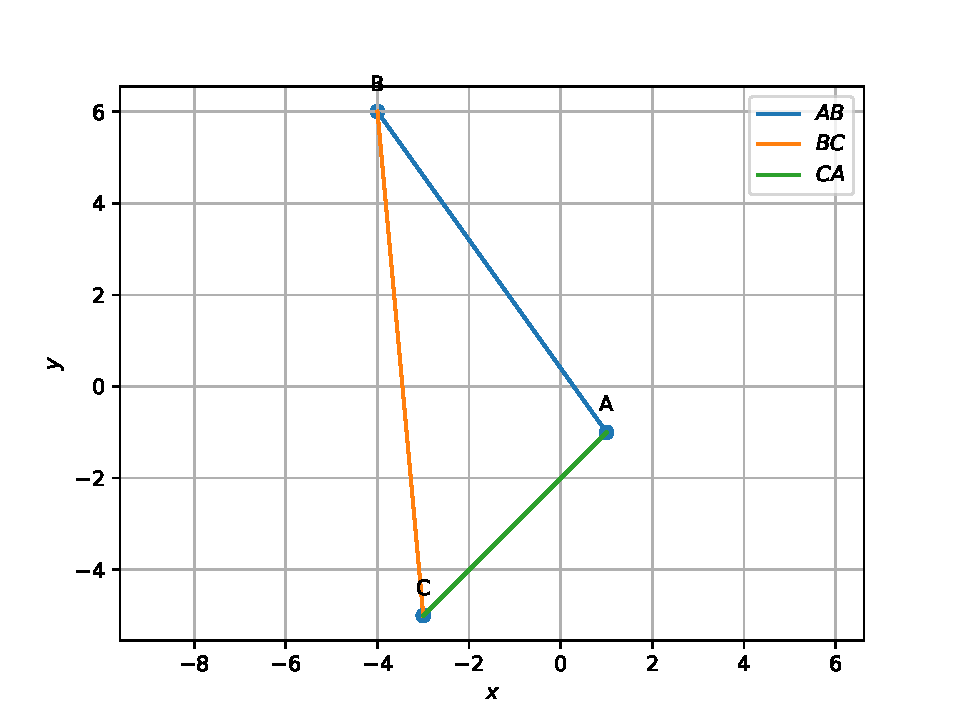
\includegraphics[width=\columnwidth]{figs/triangle/vector.pdf}
\caption{$\triangle ABC$}
\label{fig1:Triangle}
\end{figure}
% \\		\solution 
From 
			\eqref{eq:tri-pts},
\begin{align}
    \label{eq:1.1.3,2}
\myvec{
    1 & 1 & 1\\
    \vec{A} & \vec{B} & \vec{C} \\
    } 
    =
    %\label{eq:matthrowoperations}
    \myvec{
    1 & 1 & 1
    \\
    1 & -4 & -3
    \\
    -1 & 6 & -5
    }
     \xleftrightarrow[]{R_3 \leftarrow R_3+R_2}
    \myvec{
    1 & 1 & 1
    \\
    1 & -4 & -3
    \\
    0 & 2 & -8 
    }
    \\
     \xleftrightarrow[]{R_2\leftarrow R_1-R_2}
    \myvec{
    1 & 1 & 1
    \\
    0 & 5 & 4
    \\
    0 & 2 & -8 
    }
     \xleftrightarrow[]{R_3\leftarrow R_3-\frac{2}{5}R_2}
    \myvec{
    1 & 1 & 1
    \\
    0 & 5 & 4
    \\
    0 & 0 & \frac{-48}{5}
    }
\end{align}
There are no zero rows. So,
\begin{align}
    \text{rank}\myvec{
    1 & 1 & 1\\
    \vec{A} & \vec{B} & \vec{C} \\
    } &= 3 
\end{align}  
Hence,  the points $\vec{A},\vec{B},\vec{C}$ are not collinear. 
This is visible in 
\figref{fig1:Triangle}.
\begin{figure}[h]
\centering
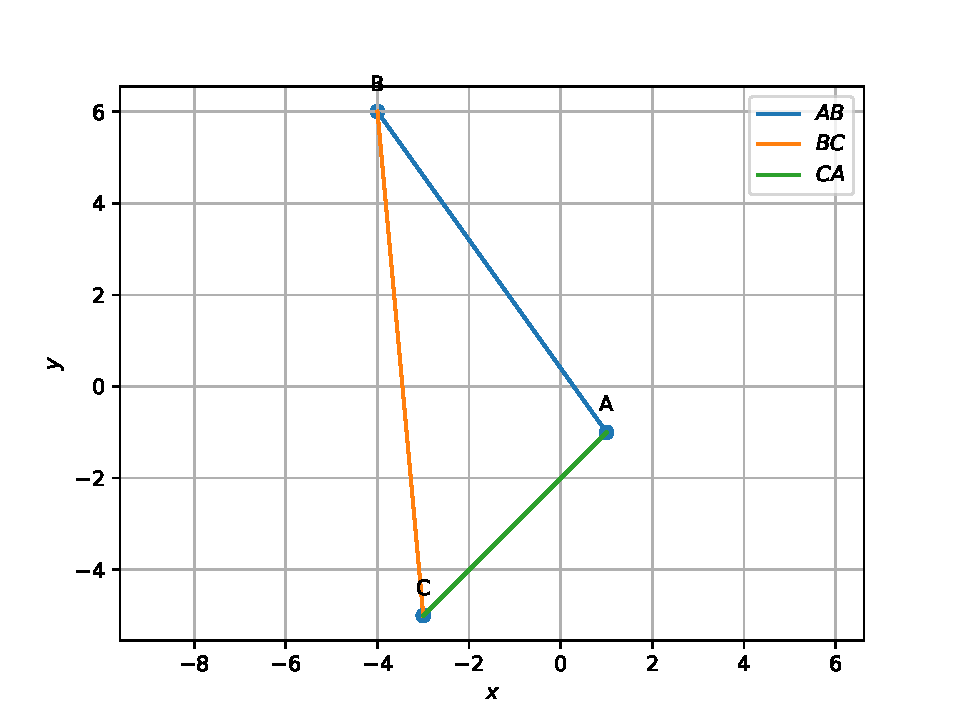
\includegraphics[width=\columnwidth]{figs/triangle/vector.pdf}
\caption{$\triangle ABC$}
\label{fig1:Triangle}
\end{figure}

\item The parameteric form of the equation  of $AB$ is 
		\begin{align}
			\label{eq:geo-param}
			\vec{x}=\vec{A}+k\vec{m} \quad k \ne 0,
		\end{align}
		where
		\begin{align}
\vec{m}=\vec{B}-\vec{A}
		\end{align}
is the direction vector of $AB$.
Find the parameteric equations of $AB, BC$ and $CA$.
\\
\solution
From 
			\eqref{eq:geo-param} and
		\eqref{eq:geo-dir-vec-ab},
the parametric equation for $AB$ is given by
\begin{align}
AB: \vec{x} = &\myvec{1\\-1} + k \myvec{-5\\7}
\end{align}
Similarly, from 
		\eqref{eq:geo-dir-vec-bc} and
		\eqref{eq:geo-dir-vec-ca},
\begin{align}
BC: \vec{x} = &\myvec{-4\\6} + k \myvec{1\\-11}\\
CA: \vec{x} = &\myvec{-3\\-5} + k \myvec{4\\4}
\end{align}

%		\solution
From 
			\eqref{eq:geo-param} and
		\eqref{eq:geo-dir-vec-ab},
the parametric equation for $AB$ is given by
\begin{align}
AB: \vec{x} = &\myvec{1\\-1} + k \myvec{-5\\7}
\end{align}
Similarly, from 
		\eqref{eq:geo-dir-vec-bc} and
		\eqref{eq:geo-dir-vec-ca},
\begin{align}
BC: \vec{x} = &\myvec{-4\\6} + k \myvec{1\\-11}\\
CA: \vec{x} = &\myvec{-3\\-5} + k \myvec{4\\4}
\end{align}


\item The normal form of the equation of $AB$  is 
		\begin{align}
			\label{eq:geo-normal}
			\vec{n}^{\top}\brak{	\vec{x}-\vec{A}} = 0
		\end{align}
		where 
		\begin{align}
			\vec{n}^{\top}\vec{m}&=\vec{n}^{\top}\brak{\vec{B}-\vec{A}} = 0
			\\
			\text{or, } \vec{n}&=\myvec{0 & 1 \\ -1 & 0} \vec{m}
			\label{eq:geo-norm-vec}
		\end{align}
Find the normal form of the equations of $AB, BC$ and $CA$.
\\
\solution
\begin{enumerate}
	\item
From
		\eqref{eq:geo-dir-vec-bc}, 
the direction vector of side $\vec{BC}$ is
\begin{align}
\vec{m}
	&=\myvec{1\\-11}
	\\
\implies \vec{n} &= \myvec{0 & 1\\
  -1 & 0}\myvec{1\\-11}
 = \myvec{-11\\-1}
		\label{eq:geo-norm-vec-bc}
\end{align}
from 
			\eqref{eq:geo-norm-vec}.
Hence, from 
			\eqref{eq:geo-normal},
the normal equation of side $BC$ is 
\begin{align}
	\vec{n}^{\top}\brak{	\vec{x}-\vec{B}} &= 0
			\\
\implies    \myvec{-11 & -1}\vec{x}&=\myvec{-11 & -1}\myvec{-4\\6}\\
    \implies
BC: \quad    \myvec{11 & 1}\vec{x}&=-38
\end{align}
\item Similarly, for $AB$,
from 
		\eqref{eq:geo-dir-vec-ab}, 
\begin{align}
	\vec{m} &= \myvec{-5\\7}
	\\
\implies        \vec{n} 
                &= \myvec{0&1\\-1&0}\myvec{-5\\7}
                = \myvec{7\\5}
		\label{eq:geo-norm-vec-ab}
\end{align}
and 
\begin{align}
	\vec{n}^{\top}\brak{	\vec{x}-\vec{A}} &= 0
	\\
	\implies
                AB: \quad  \vec{n}^{\top}\vec{x} &= \myvec{7&5}\myvec{1\\-1}\\    
       \implies\myvec{7&5}\vec{x} &= 2
\end{align}
\item For 
$CA$, 
from 
		\eqref{eq:geo-dir-vec-ca}, 
\begin{align}
\vec{m} &= \myvec{1 \\ 1}
\\
		\label{eq:geo-norm-vec-ca}
\implies \vec{n} 
&= \myvec{0&1 \\ -1&0}\myvec{1 \\ 1}
= \myvec{1 \\ -1}\\
\\
\implies	\vec{n}^{\top}\brak{	\vec{x}-\vec{C}} &= 0
\\
\implies \myvec{1&-1}{\vec{x}} &= \myvec{1&-1}\myvec{-3 \\ -5} 
= 2 
\end{align}
\end{enumerate}

%\begin{enumerate}
	\item
From
		\eqref{eq:geo-dir-vec-bc}, 
the direction vector of side $\vec{BC}$ is
\begin{align}
\vec{m}
	&=\myvec{1\\-11}
	\\
\implies \vec{n} &= \myvec{0 & 1\\
  -1 & 0}\myvec{1\\-11}
 = \myvec{-11\\-1}
		\label{eq:geo-norm-vec-bc}
\end{align}
from 
			\eqref{eq:geo-norm-vec}.
Hence, from 
			\eqref{eq:geo-normal},
the normal equation of side $BC$ is 
\begin{align}
	\vec{n}^{\top}\brak{	\vec{x}-\vec{B}} &= 0
			\\
\implies    \myvec{-11 & -1}\vec{x}&=\myvec{-11 & -1}\myvec{-4\\6}\\
    \implies
BC: \quad    \myvec{11 & 1}\vec{x}&=-38
\end{align}
\item Similarly, for $AB$,
from 
		\eqref{eq:geo-dir-vec-ab}, 
\begin{align}
	\vec{m} &= \myvec{-5\\7}
	\\
\implies        \vec{n} 
                &= \myvec{0&1\\-1&0}\myvec{-5\\7}
                = \myvec{7\\5}
		\label{eq:geo-norm-vec-ab}
\end{align}
and 
\begin{align}
	\vec{n}^{\top}\brak{	\vec{x}-\vec{A}} &= 0
	\\
	\implies
                AB: \quad  \vec{n}^{\top}\vec{x} &= \myvec{7&5}\myvec{1\\-1}\\    
       \implies\myvec{7&5}\vec{x} &= 2
\end{align}
\item For 
$CA$, 
from 
		\eqref{eq:geo-dir-vec-ca}, 
\begin{align}
\vec{m} &= \myvec{1 \\ 1}
\\
		\label{eq:geo-norm-vec-ca}
\implies \vec{n} 
&= \myvec{0&1 \\ -1&0}\myvec{1 \\ 1}
= \myvec{1 \\ -1}\\
\\
\implies	\vec{n}^{\top}\brak{	\vec{x}-\vec{C}} &= 0
\\
\implies \myvec{1&-1}{\vec{x}} &= \myvec{1&-1}\myvec{-3 \\ -5} 
= 2 
\end{align}
\end{enumerate}


\item The area of $\triangle ABC$ is defined as
		\begin{align}
			\label{eq:tri-area-cross}
			\frac{1}{2}\norm{{\brak{\vec{A}-\vec{B}}\times \brak{\vec{A}-\vec{C}}}}
		\end{align}
		where
		\begin{align}
			\vec{A}\times\vec{B} \triangleq \mydet{1 & -4 \\-1 & 6}
		\end{align}
		Find the area of $\triangle ABC$.\\
\solution
From
		\eqref{eq:geo-dir-vec-ab}
		and
		\eqref{eq:geo-dir-vec-ca},
\begin{align}
	\vec{A}-\vec{B}=\myvec{5\\-7},
	\vec{A}-\vec{C}&=\myvec{4\\4}\\
\implies (\vec{A}-\vec{B})\times(\vec{A}-\vec{C}) &=\mydet{5 & 4\\-7 & 4}\\
&=5\times 4-4\times (-7)\\&=48\\
\implies\frac{1}{2}\norm{(\vec{A}-\vec{B})\times(\vec{A}-\vec{C})}&=\frac{48}{2}=24
\end{align}
which is the desired area.

%  		\solution
From
		\eqref{eq:geo-dir-vec-ab}
		and
		\eqref{eq:geo-dir-vec-ca},
\begin{align}
	\vec{A}-\vec{B}=\myvec{5\\-7},
	\vec{A}-\vec{C}&=\myvec{4\\4}\\
\implies (\vec{A}-\vec{B})\times(\vec{A}-\vec{C}) &=\mydet{5 & 4\\-7 & 4}\\
&=5\times 4-4\times (-7)\\&=48\\
\implies\frac{1}{2}\norm{(\vec{A}-\vec{B})\times(\vec{A}-\vec{C})}&=\frac{48}{2}=24
\end{align}
which is the desired area.


	\item Find the angles $A, B, C$ if 
%    \label{prop:angle2d}
  \begin{align}
    \label{eq:angle2d}
			\cos A \triangleq 
\frac{\brak{\vec{B}-\vec{A}}^{\top}{\vec{C}-\vec{A}}}{\norm{\vec{B}-\vec{A}}\norm{\vec{C}-\vec{A}}}
  \end{align}\\
  \solution
\begin{enumerate}
	\item From 
		\eqref{eq:geo-dir-vec-ab},
		\eqref{eq:geo-dir-vec-ca},
		\eqref{eq:geo-norm-ab}
		and
		\eqref{eq:geo-norm-ca}
\begin{align}
	(\vec{B}-\vec{A})^{\top}(\vec{C}-\vec{A})&=\myvec{-5&7}\myvec{-4\\-4}\\
	&=-8
	\\
	\implies
	\cos{A}&= \frac{-8}{\sqrt{74} \sqrt{32}}
	= \frac{-1}{\sqrt{37}}\\
	\implies A&=\cos^{-1}{\frac{-1}{\sqrt{37}}}
\end{align}
	\item From 
		\eqref{eq:geo-dir-vec-ab},
		\eqref{eq:geo-dir-vec-bc},
		\eqref{eq:geo-norm-ab}
		and
		\eqref{eq:geo-norm-bc}
\begin{align}
	(\vec{C}-\vec{B})^{\top}(\vec{A}-\vec{B})&=\myvec{1&-11}\myvec{5\\-7}\\
	&= 82
	\\
	\implies
	\cos{B}&= \frac{82}{\sqrt{74} \sqrt{122}}
	= \frac{41}{\sqrt{2257}}\\
	\implies B&=\cos^{-1}{\frac{41}{\sqrt{2257}}}
\end{align}
	\item From 
		\eqref{eq:geo-dir-vec-bc},
		\eqref{eq:geo-dir-vec-ca},
		\eqref{eq:geo-norm-bc}
		and
		\eqref{eq:geo-norm-ca}
\begin{align}
	(\vec{A}-\vec{C})^{\top}(\vec{B}-\vec{C})&=\myvec{4&4}\myvec{-1\\11}\\
	&=40
	\\
\implies	\cos{C}&= \frac{40}{\sqrt{32} \sqrt{122}}
	= \frac{5}{\sqrt{61}}\\
	\implies C&=\cos^{-1}{\frac{5}{\sqrt{61}}}
\end{align}

\end{enumerate}
%  	\begin{enumerate}
	\item From 
		\eqref{eq:geo-dir-vec-ab},
		\eqref{eq:geo-dir-vec-ca},
		\eqref{eq:geo-norm-ab}
		and
		\eqref{eq:geo-norm-ca}
\begin{align}
	(\vec{B}-\vec{A})^{\top}(\vec{C}-\vec{A})&=\myvec{-5&7}\myvec{-4\\-4}\\
	&=-8
	\\
	\implies
	\cos{A}&= \frac{-8}{\sqrt{74} \sqrt{32}}
	= \frac{-1}{\sqrt{37}}\\
	\implies A&=\cos^{-1}{\frac{-1}{\sqrt{37}}}
\end{align}
	\item From 
		\eqref{eq:geo-dir-vec-ab},
		\eqref{eq:geo-dir-vec-bc},
		\eqref{eq:geo-norm-ab}
		and
		\eqref{eq:geo-norm-bc}
\begin{align}
	(\vec{C}-\vec{B})^{\top}(\vec{A}-\vec{B})&=\myvec{1&-11}\myvec{5\\-7}\\
	&= 82
	\\
	\implies
	\cos{B}&= \frac{82}{\sqrt{74} \sqrt{122}}
	= \frac{41}{\sqrt{2257}}\\
	\implies B&=\cos^{-1}{\frac{41}{\sqrt{2257}}}
\end{align}
	\item From 
		\eqref{eq:geo-dir-vec-bc},
		\eqref{eq:geo-dir-vec-ca},
		\eqref{eq:geo-norm-bc}
		and
		\eqref{eq:geo-norm-ca}
\begin{align}
	(\vec{A}-\vec{C})^{\top}(\vec{B}-\vec{C})&=\myvec{4&4}\myvec{-1\\11}\\
	&=40
	\\
\implies	\cos{C}&= \frac{40}{\sqrt{32} \sqrt{122}}
	= \frac{5}{\sqrt{61}}\\
	\implies C&=\cos^{-1}{\frac{5}{\sqrt{61}}}
\end{align}

\end{enumerate}

All codes for this section are available at
\begin{lstlisting}
	codes/triangle/sides.py
\end{lstlisting}
\end{enumerate}

\subsection{Median}
\begin{enumerate}[label=\thesubsection.\arabic*.,ref=\thesubsection.\theenumi]
\numberwithin{equation}{enumi}
\item If $\vec{D}$ divides $BC$ in the ratio $k : 1$,
		\begin{align}
			\vec{D}= \frac{k\vec{C}+\vec{B}}{k+1}
	  \label{eq:section_formula}
		\end{align}
		Find the mid points $\vec{D}, \vec{E}, \vec{F}$ of the sides $BC, CA$ and $AB$ respectively.
	\\
		\solution
Since $\vec{D}$ is the midpoint of $BC$,
\begin{align}
k &= 1,\\
\implies \vec{D} &= \frac{\vec{C} + \vec{B}}{2}
= \frac{1}{2}\myvec{-7\\1}
	\label{eq:median-d}
\end{align}
Similarly,
\begin{align}
	\label{eq:median-e}
\vec{E} &= \frac{\vec{A} + \vec{C}}{2}
= \myvec{-1\\-3}\\
\vec{F} &= \frac{\vec{A} + \vec{B}}{2}
= \frac{1}{2}\myvec{-3\\5}
	\label{eq:median-f}
\end{align}
  
	\item Find the equations of $AD, BE$ and $CF$.
	\\	\\ \solution:
\begin{enumerate}
 \item The direction vector of $AD$ is 
\begin{align}
	\vec{m} = \vec{D}- \vec{A}
&=\myvec{\frac{-7}{2}\\\frac{1}{2}} - \myvec{1\\-1}
	=\frac{1}{2}\myvec{-9\\3} \equiv \myvec{-3 \\ 1}
	\\
	\implies  \vec{n} &=\myvec{1 \\ 3}
\end{align}
Hence the normal equation of median $AD$ is 
\begin{align}
\vec{n}^{\top}\myvec{\vec{x}-\vec{A}}&=0\\
\implies    \myvec{1 & 3}\vec{x}&=\myvec{1 & 3}\myvec{1\\-1}
    =-2
	\label{eq:median-ad}
\end{align}
\item For $BE$,
\begin{align}
	\vec{m}= \vec{E}- \vec{B}&=\myvec{-1\\-3} - \myvec{-4\\6}
       =\myvec{3\\-9}
       \equiv \myvec{1\\-3}
       \\
\implies 	
\vec{n} &= 
         \myvec{3\\1}
\end{align}
Hence the normal equation of median $BE$ is 
\begin{align}
\vec{n}^{\top}\myvec{\vec{x}-\vec{B}}&=0\\
\implies
	\myvec{3 & 1}   \vec{x}&=\myvec{3 &1}\myvec{-4\\6}
    =-6
	\label{eq:median-be}
\end{align}
\item For median $CF$,
\begin{align}
	\vec{m} = \vec{F}- \vec{C} &=
\myvec{\frac{-3}{2}\\\frac{5}{2}} - \myvec{-3\\-5}
       =\myvec{\frac{3}{2}\\\frac{15}{2}}
       \equiv \myvec{1 \\ 5}
       \\
	\implies \vec{n} &=\myvec{5 \\ -1}
\end{align}
Hence the normal equation of median $CF$ is 
\begin{align}
\vec{n}^{\top}\myvec{\vec{x}-\vec{C}}&=0\\
	\implies \myvec{5 & -1}\vec{x}&=\myvec{5 & -1}\myvec{-3\\-5}
    =-10
	\label{eq:median-cf}
\end{align}
\end{enumerate}
\iffalse
\begin{figure}
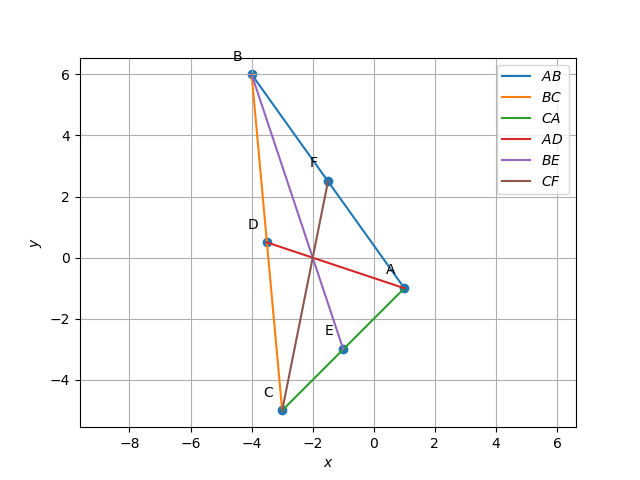
\includegraphics [width=\columnwidth] {solutions/1/2/2/figs/figure.png}
\caption{ Medians $AD$ , $BE$ and $CF$}
\label{fig: medians}
\end{figure}
\fi




% 		\iffalse
\let\negmedspace\undefined
\let\negthickspace\undefined
\documentclass[journal,12pt,twocolumn]{IEEEtran}
\usepackage{cite}
\usepackage{amsmath,amssymb,amsfonts,amsthm}
\usepackage{algorithmic}
\usepackage{graphicx}
\usepackage{textcomp}
\usepackage{xcolor}
\usepackage{txfonts}
\usepackage{listings}
\usepackage{enumitem}
\usepackage{mathtools}
\usepackage{gensymb}
\usepackage[breaklinks=true]{hyperref}
\usepackage{tkz-euclide} % loads  TikZ and tkz-base
\usepackage{listings}
\usepackage{gvv}
%
%\usepackage{setspace}
%\usepackage{gensymb}
%\doublespacing
%\singlespacing

%\usepackage{graphicx}
%\usepackage{amssymb}
%\usepackage{relsize}
%\usepackage[cmex10]{amsmath}
%\usepackage{amsthm}
%\interdisplaylinepenalty=2500
%\savesymbol{iint}
%\usepackage{txfonts}
%\restoresymbol{TXF}{iint}
%\usepackage{wasysym}
%\usepackage{amsthm}
%\usepackage{iithtlc}
%\usepackage{mathrsfs}
%\usepackage{txfonts}
%\usepackage{stfloats}
%\usepackage{bm}
%\usepackage{cite}
%\usepackage{cases}
%\usepackage{subfig}
%\usepackage{xtab}
%\usepackage{longtable}
%\usepackage{multirow}
%\usepackage{algorithm}
%\usepackage{algpseudocode}
%\usepackage{enumitem}
%\usepackage{mathtools}
%\usepackage{tikz}
%\usepackage{circuitikz}
%\usepackage{verbatim}
%\usepackage{tfrupee}
%\usepackage{stmaryrd}
%\usetkzobj{all}
%    \usepackage{color}                                            %%
%    \usepackage{array}                                            %%
%    \usepackage{longtable}                                        %%
%    \usepackage{calc}                                             %%
%    \usepackage{multirow}                                         %%
%    \usepackage{hhline}                                           %%
%    \usepackage{ifthen}                                           %%
  %optionally (for landscape tables embedded in another document): %%
%    \usepackage{lscape}     
%\usepackage{multicol}
%\usepackage{chngcntr}
%\usepackage{enumerate}

%\usepackage{wasysym}
%\documentclass[conference]{IEEEtran}
%\IEEEoverridecommandlockouts
% The preceding line is only needed to identify funding in the first footnote. If that is unneeded, please comment it out.

\newtheorem{theorem}{Theorem}[section]
\newtheorem{problem}{Problem}
\newtheorem{proposition}{Proposition}[section]
\newtheorem{lemma}{Lemma}[section]
\newtheorem{corollary}[theorem]{Corollary}
\newtheorem{example}{Example}[section]
\newtheorem{definition}[problem]{Definition}
%\newtheorem{thm}{Theorem}[section] 
%\newtheorem{defn}[thm]{Definition}
%\newtheorem{algorithm}{Algorithm}[section]
%\newtheorem{cor}{Corollary}
\newcommand{\BEQA}{\begin{eqnarray}}
\newcommand{\EEQA}{\end{eqnarray}}
\newcommand{\define}{\stackrel{\triangle}{=}}
\theoremstyle{remark}
\newtheorem{rem}{Remark}

%\bibliographystyle{ieeetr}
\begin{document}
%

\bibliographystyle{IEEEtran}


\vspace{3cm}

\title{ Solution of 1.2.2
%	\logo{

%	}
}
\author{ Dhruv Parashar$^{*}$% <-this % stops a space
	
}	
%\title{
%	\logo{Matrix Analysis through Octave}{\begin{center}\includegraphics[scale=.24]{tlc}\end{center}}{}{HAMDSP}
%}


% paper title
% can use linebreaks \\ within to get better formatting as desired
%\title{Matrix Analysis through Octave}
%
%
% author names and IEEE memberships
% note positions of commas and nonbreaking spaces ( ~ ) LaTeX will not break
% a structure at a ~ so this keeps an author's name from being broken across
% two lines.
% use \thanks{} to gain access to the first footnote area
% a separate \thanks must be used for each paragraph as LaTeX2e's \thanks
% was not built to handle multiple paragraphs
%

%\author{<-this % stops a space
%\thanks{}}
%}
% note the % following the last \IEEEmembership and also \thanks - 
% these prevent an unwanted space from occurring between the last author name
% and the end of the author line. i.e., if you had this:
% 
% \author{....lastname \thanks{...} \thanks{...} }
%                     ^------------^------------^----Do not want these spaces!
%
% a space would be appended to the last name and could cause every name on that
% line to be shifted left slightly. This is one of those "LaTeX things". For
% instance, "\textbf{A} \textbf{B}" will typeset as "A B" not "AB". To get
% "AB" then you have to do: "\textbf{A}\textbf{B}"
% \thanks is no different in this regard, so shield the last } of each \thanks
% that ends a line with a % and do not let a space in before the next \thanks.
% Spaces after \IEEEmembership other than the last one are OK (and needed) as
% you are supposed to have spaces between the names. For what it is worth,
% this is a minor point as most people would not even notice if the said evil
% space somehow managed to creep in.



% The paper headers
%\markboth{Journal of \LaTeX\ Class Files,~Vol.~6, No.~1, January~2007}%
%{Shell \MakeLowercase{\textit{et al.}}: Bare Demo of IEEEtran.cls for Journals}
% The only time the second header will appear is for the odd numbered pages
% after the title page when using the twoside option.
% 
% *** Note that you probably will NOT want to include the author's ***
% *** name in the headers of peer review papers.                   ***
% You can use \ifCLASSOPTIONpeerreview for conditional compilation here if
% you desire.




% If you want to put a publisher's ID mark on the page you can do it like
% this:
%\IEEEpubid{0000--0000/00\$00.00~\copyright~2007 IEEE}
% Remember, if you use this you must call \IEEEpubidadjcol in the second
% column for its text to clear the IEEEpubid mark.



% make the title area
\maketitle

\newpage

%\tableofcontents

\bigskip

\renewcommand{\thefigure}{\theenumi}
\renewcommand{\thetable}{\theenumi}
%\renewcommand{\theequation}{\theenumi}

%\begin{abstract}
%%\boldmath
%In this letter, an algorithm for evaluating the exact analytical bit error rate  (BER)  for the piecewise linear (PL) combiner for  multiple relays is presented. Previous results were available only for upto three relays. The algorithm is unique in the sense that  the actual mathematical expressions, that are prohibitively large, need not be explicitly obtained. The diversity gain due to multiple relays is shown through plots of the analytical BER, well supported by simulations. 
%
%\end{abstract}
% IEEEtran.cls defaults to using nonbold math in the Abstract.
% This preserves the distinction between vectors and scalars. However,
% if the journal you are submitting to favors bold math in the abstract,
% then you can use LaTeX's standard command \boldmath at the very start
% of the abstract to achieve this. Many IEEE journals frown on math
% in the abstract anyway.

% Note that keywords are not normally used for peerreview papers.
%\begin{IEEEkeywords}
%Cooperative diversity, decode and forward, piecewise linear
%\end{IEEEkeywords}



% For peer review papers, you can put extra information on the cover
% page as needed:
% \ifCLASSOPTIONpeerreview
% \begin{center} \bfseries EDICS Category: 3-BBND \end{center}
% \fi
%
% For peerreview papers, this IEEEtran command inserts a page break and
% creates the second title. It will be ignored for other modes.
%\IEEEpeerreviewmaketitle


Question:- 
We are given the three vertices of a triangle$(A,B,C)$ and the midpoints $\vec{D},\vec{E},\vec{F}$ of the sides $AB,BC,AC$ respectively. We have to find the equations of the sides $AD,BE,CF$.
\\
\fi
\solution
\begin{align}
\vec{A} &= \myvec{1\\-1} \\
\vec{B} &= \myvec{-4\\6} \\
\vec{C} &= \myvec{-3\\-5}
\end{align}
The mid points $\vec{D},\vec{E},\vec{F}$ of sides $AB,BC,AC$ are :-
\begin{align}
\vec{D} &= \frac{1}{2}\myvec{-7  \\ 1}\\
\vec{E} &= \myvec{-1\\-3}\\
\vec{F} &= \frac{1}{2}\myvec{-3  \\ 5}
\end{align}
Now, the direction vector of line $FC(\vec{m})$ is :-
\begin{align}
\vec{m} &= \vec{F} - \vec{C} \\
\implies \vec{m} &= \frac{1}{2}\myvec{3 \\ 15}
\end{align}
Now, we have to find $\vec{n}$,
\begin{align}
\vec{n} &= \myvec{0 & 1 \\ -1 & 0}\vec{m}\\
&= \frac{1}{2}\myvec{0 & 1 \\ -1 & 0}\myvec{3\\15}\\
&=\frac{1}{2}\myvec{15\\-3}
\end{align}
Normal form of line CF is :
\begin{align}
\vec{n}^{\top}(\vec{x-C}) &= 0\\
\vec{n}^{\top}\vec{x} &= \vec{n}^{\top}\vec{C} \\
\frac{1}{2}\myvec{15 & -3}\vec{x} &= \frac{1}{2}\myvec{15 & -3}\myvec{-3\\-5} \\
\myvec{15 & -3}\vec{x} &= \myvec{15 & -3}\myvec{-3\\-5} \\
\myvec{15 & -3}\vec{x} &= -30
\end{align}

\begin{figure}
\centering
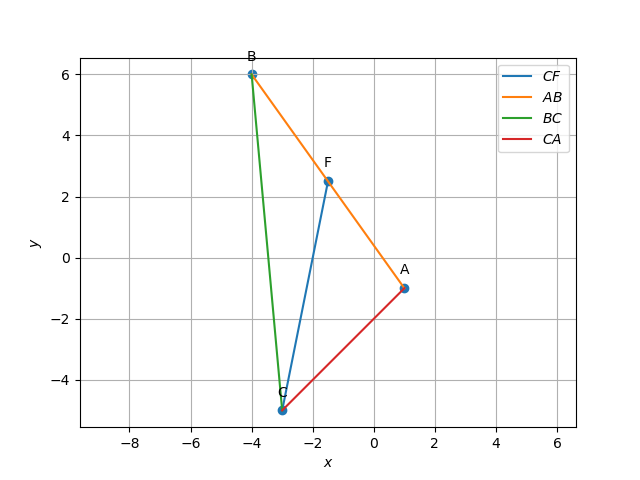
\includegraphics[width=\columnwidth]{solutions/1/2/2a/figs/figure.png}
\caption{Line CF}
\label{fig:Line CF}
\end{figure}



	\item Find the intersection $\vec{G}$ of $BE$ and $CF$.
 \\
\solution 
From 
	\eqref{eq:median-be}
	and
	\eqref{eq:median-cf},
the equations of $BE$ 
and 
$CF$
are, respectively,
\begin{align}
\myvec{3 & 1} \vec{x} &= \myvec{-6}
\label{eq:1.2.3,8}
\\
\myvec{ 5&-1} \vec{x} &= \myvec{-10}
\label{eq:1.2.3,9}
\end{align}
From \eqref{eq:1.2.3,8} and \eqref{eq:1.2.3,9} the augmented matrix is
\begin{align}
    \label{eq:matrowoperations}
    \myvec{
    3 & 1 & -6
    \\
    5 & -1 & -10
    }
     \xleftrightarrow[]{R_1 \leftarrow R_1+R_2}
    \myvec{
    8 & 0 & -16
    \\
    5 & -1 & -10 
    }
    \\
     \xleftrightarrow[]{R_1\leftarrow R_1/8}
    \myvec{
    1 & 0 & -2
    \\
    5 & -1 & -10 
    }
     \xleftrightarrow[]{R_2\leftarrow R_2-5R_1}
    \myvec{
    1 & 0 & -2
    \\
    0 & -1 & 0
    }
    \\
     \xleftrightarrow[]{R_2\leftarrow -R_2}
    \myvec{
    1 & 0 & -2
    \\
    0 & 1 & 0
    }
\end{align} 
using Gauss elimination.  Therefore, 
\begin{align}
\vec{G} = \myvec{-2 \\ 0}
	\label{eq:median-g}
\end{align}

	\item Verify that 
		\begin{align}
			\frac{BG}{GE} = 
			\frac{CG}{GF} =
			\frac{AG}{GD} =2 
		\end{align}
		\\	\solution 
\begin{enumerate}
\item From 
	\eqref{eq:median-e}
	and
	\eqref{eq:median-g},
\begin{align}
		\label{eq:tri-pts/4} \vec{G}-\vec{B} &= \myvec{2 \\ -6},\, 
 \vec{E}-\vec{G} = \myvec{1 \\ -3} \\
	\implies \vec{G}-\vec{B} &= 2 \brak{ \vec{E}-\vec{G} }
	\\
	\implies \norm{\vec{G}-\vec{B}} &= 2 \norm{ \vec{E}-\vec{G} }
	\\
	\text{or, }		\label{eq:tri-pts/8}\frac{BG}{GE} &=  2  
\end{align}		
\item From 
	\eqref{eq:median-f}
	and
	\eqref{eq:median-g},
\begin{align}
		 \vec{F}-\vec{G} &= \frac{1}{2}\myvec{ 1 \\ 5},\, 
 \vec{G}-\vec{C} &= \myvec{1 \\ 5} \\
	\implies 		 \vec{G}-\vec{C} &= 2 \brak{\vec{F}-\vec{G}} 
	\\
	\implies 		 \norm{\vec{G}-\vec{C}} &= 2 \norm{\vec{F}-\vec{G}} 
	\\
		\text{or, }	\frac{CG}{GF} &=  2		
\label{eq:tri-pts/9}
\end{align}
\item From
	\eqref{eq:median-d}
	and
	\eqref{eq:median-g},
\begin{align}
		\label{eq:tri-pts/14} \vec{G}-\vec{A} &= \myvec{-3 \\ 1} ,\,
 \vec{D}-\vec{G} = \frac{1}{2}\myvec{ -3 \\ 1}
 \\
	\vec{G}-\vec{A} &= 
	2\brak{ \vec{D}-\vec{G} } 
	\\
\implies		 \norm{\vec{G}-\vec{A}} &= 
 2\norm{\vec{D}-\vec{G}} 
 \\
		\text{or, }		\label{eq:tri-pts/18}\frac{AG}{GD} &=   2		
\end{align}
\end{enumerate}
From \eqref{eq:tri-pts/8}, \eqref{eq:tri-pts/9}, \eqref{eq:tri-pts/18}
\begin{align}
		\frac{BG}{GE} = 
		\frac{CG}{GF} =
		\frac{AG}{GD} = 2
\end{align}

	\item Show that $\vec{A}, \vec{G}$ and $\vec{D}$ are collinear.
	\\
		\solution 
Points $\vec{A},\vec{D},\vec{G}$ are defined to be collinear if 
\begin{align}
    \text{rank}\myvec{
    1 & 1 & 1\\
    \vec{A} & \vec{D} & \vec{G} \\
    } = 2 
    \label{eq:mat_row_operations}
    \\
\implies    
    \myvec{
    1 & 1 & 1
    \\
    1 & -\frac{7}{2} & -2
    \\
    -1 & \frac{1}{2} & 0
    }
     \xleftrightarrow[]{R_3 \leftarrow R_3+R_2}
    \myvec{
    1 & 1 & 1
    \\
    1 & -\frac{7}{2} & -2
    \\
    0 & -3 & -2 
    }
    \\
     \xleftrightarrow[]{R_2\leftarrow R_2-R_1}
    \myvec{
    1 & 1 & 1
    \\
    0 & -\frac{9}{2} & -3
    \\
    0 & -3 & -2 
    }
     \xleftrightarrow[]{R_3\leftarrow R_3-\frac{2}{3}R_2}
    \myvec{
    1 & 1 & 1
    \\
    0 & -\frac{9}{2} & -3
    \\
    0 & 0 & 0
    }
\end{align}
Thus, the matrix 
    \eqref{eq:mat_row_operations}
    has rank 2 and the points are collinear.
    Thus, the medians of a triangle meet at the point $\vec{G}$.
See \figref{fig:Triangle-median}.
\begin{figure}
\centering
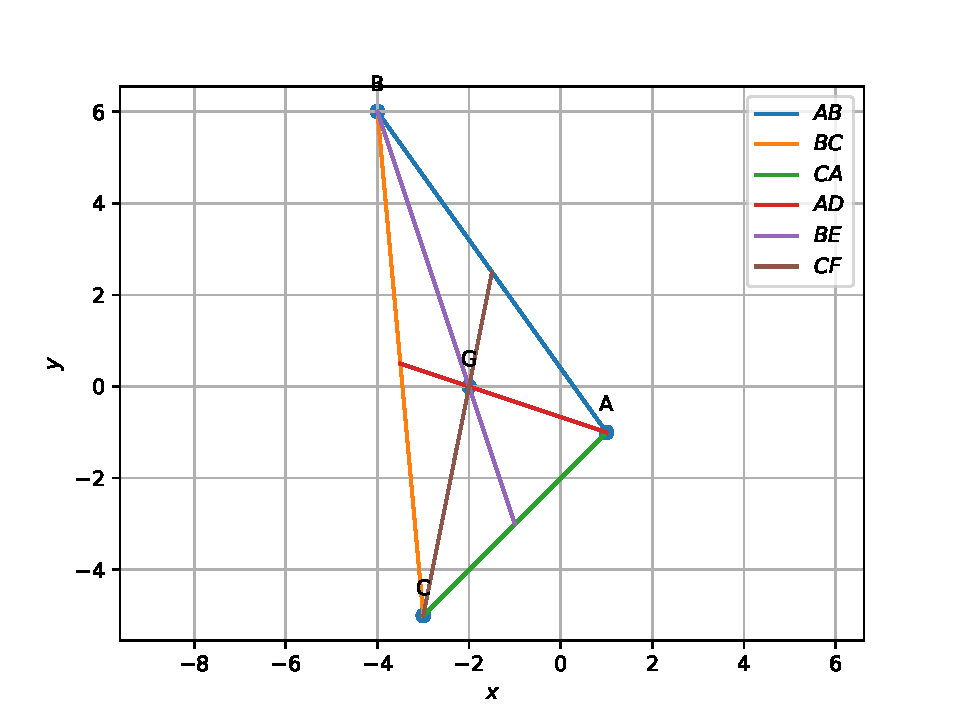
\includegraphics[width=\columnwidth]{figs/triangle/median.pdf}
	\caption{Medians of $\triangle ABC$ meet at $\vec{G}$.}
\label{fig:Triangle-median}
\end{figure}


	\item Verify that 
		\begin{align}
			\vec{G}=\frac{\vec{A}+\vec{B}+\vec{C}}{3}
		\end{align}
			$\vec{G}$ is known as the {\em centroid} of $\triangle ABC$.
   \\
		\solution
\begin{equation}
\begin{split}
\label{eq:centroid}
    \vec{G}&= \frac{\myvec{1\\-1}+\myvec{-4\\6}+\myvec{-3\\-5}}{3}\\    
     &= \myvec{-2\\0}
\end{split}
\end{equation}

 




	\item Verify that 
		\begin{align}
\vec{A}-\vec{F}=\vec{E}-\vec{D}
		\end{align}
		The quadrilateral $AFDE$ is defined to be a parallelogram.\\
  		\\ \solution 
\begin{align}
    \vec{A}-\vec{F}&=\myvec{1\\-1}-\myvec{\frac{-3}{2}\\\frac{5}{2}}
    =\myvec{\frac{5}{2}\\\frac{-7}{2}}
    \\
    \vec{E}-\vec{D}&=\myvec{-1\\-3}-\myvec{\frac{-7}{2}\\\frac{1}{2}}
    =\myvec{\frac{5}{2}\\\frac{-7}{2}}
    \\
	\implies	\vec{A}-\vec{F} &= \vec{E}-\vec{D}
\end{align}
See \figref{fig:Triangle-pgm}, 
\begin{figure}
\centering
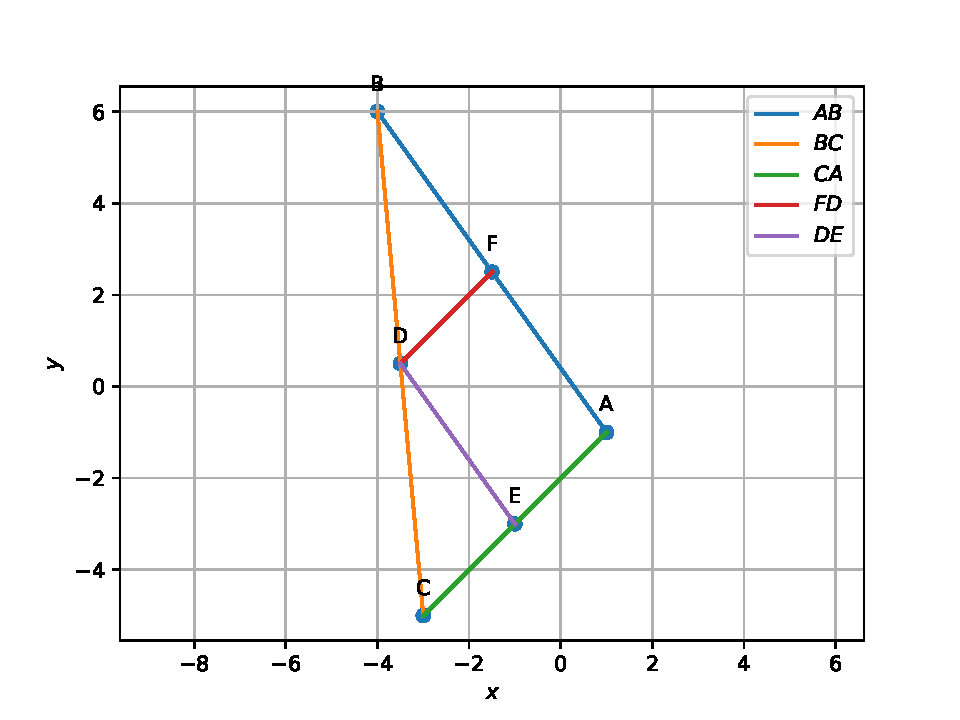
\includegraphics[width=\columnwidth]{figs/triangle/pgm.pdf}
\caption{$AFDE$ forms a parallelogram in triangle ABC}
\label{fig:Triangle-pgm}
\end{figure}






















All codes for this section are available in 
\begin{lstlisting}
	codes/triangle/medians.py
	codes/triangle/pgm.py
\end{lstlisting}
  
\end{enumerate}

\subsection{Altitude}
\begin{enumerate}[label=\thesubsection.\arabic*.,ref=\thesubsection.\theenumi]
\numberwithin{equation}{enumi}
\numberwithin{figure}{enumi}
\item $\vec{D}_1$ is a point on $BC$ such that
		\begin{align}
			AD_1 \perp BC
		\end{align}
		and $AD_1$ is defined to be the altitude. 
		Find the normal vector of $AD_1$.
  \\
		\solution
The normal vector of $AD_{1}$ 
is
the direction vector $BC$ and is obtained from  
		\eqref{eq:geo-dir-vec-bc}
		as
\begin{align}
	\vec{n} = 
\myvec{1\\-11}
\end{align}


	\item Find the equation of $AD_1$.
 \\     \solution
The equation of $AD_1$ is
\begin{align}
 \vec{n}^{\top}(\vec{x-A}) &= 0 \\
\implies \myvec{-1 & 11}\vec{x} &= \myvec{-1 & 11}\myvec{1 \\ -1}
= -12
\end{align}


	\item Find the equations of the altitudes $BE_1$ and $CF_1$ to the sides $AC$ and $AB$ respectively. 
  \\     \\ \solution
\begin{enumerate}
\item 
	From 
		\eqref{eq:geo-dir-vec-ca},
the normal vector of $CF_1$ is 
\begin{align}
\vec{n}&=\myvec{-5\\7} 
\end{align}
and the equation of $CF_1$ is
\begin{align}
\vec{n}^{\top}\brak{\vec{x}-\vec{C}}&=0 \\
\implies 
\myvec{-5 & 7}\brak{\vec{x}-\myvec{-3\\-5}}&=0  \\
	\implies \myvec{5 & -7}\vec{x}&=20
		\label{eq:geo-alt-cf},
\end{align}
\item Similarly, 
	from 
		\eqref{eq:geo-dir-vec-ab},
the normal vector of $BE_1$ is 
\begin{align}
\vec{n}= \myvec{1 \\1}
\end{align}
and the equation of  $BE_1$ is
\begin{align}
\vec{n}^{\top}\brak{\vec{x}-\vec{B}}&=0 \\
	\implies \myvec{1 & 1}\brak{\vec{x}-\myvec{-4\\6}}&=0 \\
	\implies \myvec{1 & 1}\vec{x}&=2
		\label{eq:geo-alt-be},
\end{align}
\end{enumerate}



	\item Find the intersection $\vec{H}$ of $BE_1$ and $CF_1$.
 \\
        \\ \solution
%
The intersection of 
		\eqref{eq:app-geo-alt-be}
		and
		\eqref{eq:app-geo-alt-cf},
		is obtained from 
		the matrix equation
		%
\begin{align}
        \myvec{1&1\\5&-7} \vec{x} &= \myvec{2\\20}
\end{align}
%
which can be solved as 
%
\begin{align}
        \myvec{1&1&2\\5&-7&20}
	 \xleftrightarrow[]{R_2 \leftarrow R_2 - 5R_1}
        \myvec{1&1&2\\0&-12&10}\\
	 \xleftrightarrow[]{R_2 \leftarrow \frac{R_2}{-12}}
        \myvec{1&1&2\\0&1&\frac{-5}{6}}
	 \xleftrightarrow[]{R_1 \leftarrow R_1 - R_2}
        \myvec{1&0&\frac{17}{6}\\0&1&\frac{-5}{6}}
\end{align}
%
yielding
%
\begin{align}
        \vec{H}&=\frac{1}{6}\myvec{{17}\\-{5}}
		\label{eq:app-geo-alt-H},
\end{align}
%
See 
\figref{fig:m_tri_py}
\begin{figure}[H]
\centering
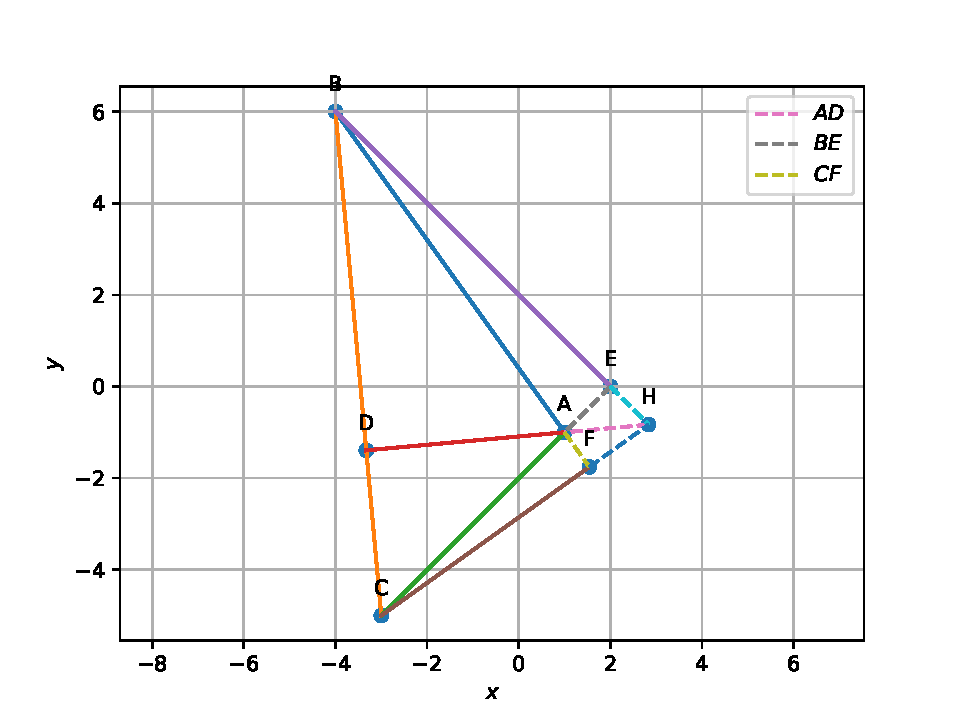
\includegraphics[width=0.75\columnwidth]{figs/triangle/altitude.pdf}
\caption{Altitudes $BE_1$ and $CF_1$ intersect at $\vec{H}$}
\label{fig:m_tri_py}
\end{figure}


	\item Verify that 
		\begin{align}
			\brak{\vec{A}-\vec{H}}^{\top}\brak{\vec{B}-\vec{C}} = 0
		\end{align}
  \solution
From 
		\eqref{eq:geo-alt-H},
\begin{align}
\vec{A}-\vec{H}=-\frac{1}{6}\myvec{{11}\\{1}},\,
\vec{B}-\vec{C}=\myvec{-1\\11}
\\
	\implies \brak{\vec{A}-\vec{H}}^{\top}\brak{\vec{B}-\vec{C}}=\frac{1}{6}\myvec{11 & 1}
\myvec{-1\\11}
=0
\end{align}


All codes for this section are available at
\begin{lstlisting}
	codes/triangle/altitude.py
\end{lstlisting}
\end{enumerate}

\subsection{Perpendicular Bisector}
\begin{enumerate}[label=\thesubsection.\arabic*.,ref=\thesubsection.\theenumi]
\numberwithin{equation}{enumi}

\item The equation of the perpendicular bisector of $BC$ is
		\begin{align}
			\label{eq:tri-perp-bisect}
			\brak{\vec{x}-\frac{\vec{B}+\vec{C}}{2}}\brak{\vec{B}-\vec{C}} = 0
		\end{align}
		Substitute numerical values and find the equations of the perpendicular bisectors of $AB, BC$ and $CA$.
	\\	\solution
From 
		\eqref{eq:app-geo-dir-vec-ab},
		\eqref{eq:app-geo-dir-vec-bc},
		\eqref{eq:app-geo-dir-vec-ca},
	\eqref{eq:median-d},
	\eqref{eq:median-e}
	and
	\eqref{eq:median-f},
\begin{align}
\vec{\frac{\vec{B}+\vec{C}}{2}} &= \frac{1}{2}\myvec{-{7} \\ 1},\,
\vec{B}-\vec{C} = \myvec{-1 \\ 11} 
\\
\vec{\frac{\vec{A}+\vec{B}}{2}}&=\frac{1}{2}\myvec{-{3} \\{5}},\,
\vec{A}-\vec{B}=\myvec{5\\ -7} \\
\vec{\frac{\vec{C}+\vec{A}}{2}} &= \myvec{-1\\-3},\,
\vec{C}-\vec{A} = \myvec{-4\\-4} 
\end{align}
yielding
\begin{alignat}{2}
  \brak{\vec{B}-\vec{C}}^{\top}\brak{\frac{\vec{B}+\vec{C}}{2}}
	&=\myvec{-1&11}\myvec{-\frac{7}{2} \\ \frac{1}{2}}
	&&=9
  \\
\brak{\vec{A}-\vec{B}}^{\top}\brak{\frac{\vec{A}+\vec{B}}{2}}
	&=\myvec{5&-7}\myvec{-\frac{3}{2} \\\frac{5}{2}}
	&&=-25
  \\
\brak{\vec{C}-\vec{A}}^{\top}\brak{\frac{\vec{C}+\vec{A}}{2}}
	&=\myvec{-4&-4}\myvec{-1\\-3}
	&&=16
\end{alignat}
Thus, the perpendicular bisectors are obtained from 
			\eqref{eq:tri-perp-bisect}
			as
		\begin{alignat}{2}
			\label{eq:app-tri-perp-bisect-bc}
			BC&: \quad \myvec{-1&11}\vec{x}&&=9
\\
			\label{eq:app-tri-perp-bisect-ca}
			CA&: \quad \myvec{5&-7}\vec{x}&&=-25
\\
			\label{eq:app-tri-perp-bisect-ab}
			AB&: \quad \myvec{1&1}\vec{x}&&=-4
		\end{alignat}




	\item Find the intersection $\vec{O}$ of the perpendicular bisectors of $AB$ and $AC$.
 \\
 \solution \\
The intersection of 
			\eqref{eq:app-tri-perp-bisect-ca}
			and
			\eqref{eq:app-tri-perp-bisect-ab},
			can be obtained as
\begin{align}
\myvec{5&-7&-25\\1&1&-4} \xleftrightarrow[]{R_2 \leftarrow 5R_2 - R_1} \myvec{5&-7&-25\\0&12&5}\\
 \xleftrightarrow[]{R_1\leftarrow \frac{12}{7}R_1 + R_2} \myvec{\frac{60}{7}&0& \frac{-265}{7}\\0&12&5}
 \xleftrightarrow[R_1\leftarrow \frac{7}{60}R_1]{R_2 \leftarrow \frac{1}{12}R_2} \myvec{1&0& \frac{-53}{12}\\0&1&\frac{5}{12}}\\
\implies \vec{O}=\myvec{\frac{-53}{12}\\\frac{5}{12}}
			\label{eq:app-tri-perp-bisect-O}
\end{align}

	\item Verify that $\vec{O}$ satisfies
			\eqref{eq:tri-perp-bisect}.
$\vec{O}$ is known as the circumcentre.\\
    \solution
Substituing  from 
			\eqref{eq:tri-perp-bisect-O} in 
			\eqref{eq:tri-perp-bisect},
when substituted in the above equation,
\begin{multline}
	\brak{\vec{O}-\frac{\vec{B}+\vec{C}}{2}}^{\top}\brak{\vec{B}-\vec{C}}\\
	=\brak{\frac{1}{12}\myvec{-53\\5}- \frac{1}{2}\myvec{-7\\1}}^{\top} \myvec{-1\\11}\\
	=\frac{1}{12}\myvec{-11&-1}\myvec{-1\\11}
	=0
\end{multline}




		\item Verify that 
		\begin{align}
			OA = OB = OC 
		\end{align}
	\item Draw the circle with centre at $\vec{O}$ and radius 
		\begin{align}
			R = OA
		\end{align}
		This is known as the {\em circumradius}. 
  \\  \solution 
See 
\figref{fig:circumcircle with centre O}.
\begin{figure}
\centering
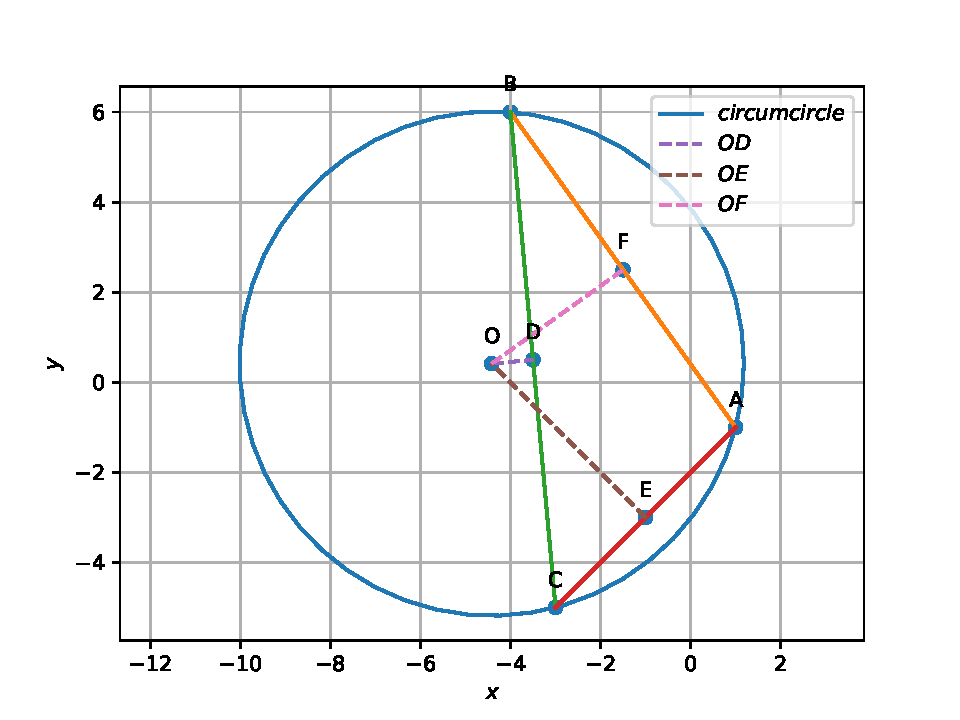
\includegraphics[width=0.75\columnwidth]{figs/triangle/perp-bisect.pdf}
	\caption{Circumcircle of $\triangle ABC$ with centre $\vec{O}$.}
\label{fig:circumcircle with centre O}	
\end{figure}


	\item Verify that 
		\begin{align}
			\angle BOC = 2\angle BAC.
		\end{align}\\
  \solution
\begin{enumerate}
\item To find  the value of $\angle{BOC}$ :
\begin{align}
\vec{B}-\vec{O}
          &=\myvec{\frac{5}{12}\\\frac{67}{12}},\,
\vec{C}-\vec{O}
          =\myvec{\frac{17}{12}\\\frac{-65}{12}}
	  \\
\implies \brak{\vec{B}-\vec{O}}^{\top}\brak{\vec{C}-\vec{O}}&=\frac{-4270}{144}\\
	\implies \norm{\vec{B}-\vec{O}}&= \frac{\sqrt{4514}}{12},\,
	\norm{\vec{C}-\vec{O}}= \frac{\sqrt{4514}}{12}
\end{align}
Thus,
\begin{align}
\cos{BOC}&=\frac{\brak{\vec{B}-\vec{O}}^{\top}\brak{\vec{C}-\vec{O}}}{\norm{\vec{B}-\vec{O}}\norm{\vec{C}-\vec{O}}}
=\frac{-4270}{4514}\\
\implies\angle{BOC}&=\cos^{-1}\brak{\frac{-4270}{4514}}
\\
	&=161.07536\degree
	\text{ or }
	198.92464\degree\label{eq:1}
\end{align}
	\item To find  the value of $\angle{BAC}$ :
\begin{align}
\vec{B}-\vec{A}&=\myvec{-5\\7},\,
\vec{C}-\vec{A}=\myvec{-4\\-4}
\\
\implies \brak{\vec{B}-\vec{A}}^{\top}\brak{\vec{C}-\vec{A}}&=-8
\\
	\norm{\vec{B}-\vec{A}}&= \sqrt{74}
	\norm{\vec{C}-\vec{A}}= 4\sqrt{2}
\end{align}
Thus,
\begin{align}
\cos{BAC}&=\frac{\brak{\vec{B}-\vec{A}}^{\top}\brak{\vec{C}-\vec{A}}}{\norm{\vec{B}-\vec{A}}\norm{\vec{C}-\vec{A}}}
=\frac{-8}{4\sqrt{148}}\\
\implies\angle{BAC}&=\cos^{-1}\brak{\frac{-8}{4\sqrt{148}}}\\
&=99.46232\degree \label{eq:2}
\end{align}
From \eqref{eq:2} and \eqref{eq:1},
\begin{align}
2\times\angle{BAC}
= \angle{BOC}
\end{align}
\end{enumerate}





	\item Let 
		\begin{align}
			\vec{P} = \myvec{\cos \theta & -\sin \theta \\ \sin \theta & \cos \theta}
		\end{align}
			where
\begin{align}
	\theta = \angle BOC
\end{align}
Verify that 
		\begin{align}
			\vec{B}-\vec{O}=\vec{P}\brak{\vec{C}-\vec{O}}
		\end{align}
All codes for this section are available at
\begin{lstlisting}
	codes/triangle/perp-bisect.py
\end{lstlisting}
\end{enumerate}

\subsection{Angle Bisector}
\begin{enumerate}[label=\thesubsection.\arabic*.,ref=\thesubsection.\theenumi]
\numberwithin{equation}{enumi}
\numberwithin{figure}{enumi}
	\item Let $\vec{D}_3, \vec{E}_3, \vec{F}_3$, be points on $AB, BC$ and $CA$ respectively such that
		\begin{align}
			BD_3 = BF_3=m, CD_3 = CE_3=n, AE_3 = AF_3=p.
		\end{align}
	Obtain $m,n,p$ in terms of $a,b,c$ obtained in  
		\probref{prob:side-length}.
 \\
 		\solution 
From the given information, 
\begin{align}
% 
    a &= m+n,\\
    b &= n+p, \\
    c &= m+p 
\end{align}
which can be expressed as
\begin{align}
\myvec{1&1&0\\0&1&1\\1&0&1\\}\myvec{m\\n\\p} &= \myvec{a\\b\\c}
\\
\implies 
	\myvec{m\\n\\p} &= \myvec{1&1&0\\0&1&1\\1&0&1\\}^{-1}\myvec{a\\b\\c}
\end{align}
Using row reduction,
		\begin{align}
			\augvec{3}{3}{1&1&0 & 1 & 0 & 0\\0&1&1 & 0 & 1 & 0\\1&0&1 & 0 & 0 & 1}
			\\
			\xleftrightarrow[]{R_3 \leftarrow R_3 - R_1}
			\augvec{3}{3}{1&1&0 & 1 & 0 & 0\\0&1&1 & 0 & 1 & 0\\0&-1&1 & -1 & 0 & 1}
			\\
			\xleftrightarrow[R_1 \leftarrow R_1 - R_2]{R_3 \leftarrow R_3 + R_2}
			\augvec{3}{3}{1&0&-1 & 1 & -1 & 0\\0&1&1 & 0 & 1 & 0\\0&0&2 & -1 & 1 & 1}
		\end{align}
		\begin{align}
			\xleftrightarrow[R_1 \leftarrow 2R_1 + R_3]{R_2 \leftarrow 2R_2 - R_3}
			\augvec{3}{3}{2&0&0 & 1 & -1 & 1\\0&2&0 & 1 & 1 & -1\\0&0&2 & -1 & 1 & 1}
		\end{align}
yielding
		\begin{align}
			\myvec{1&1&0\\0&1&1\\1&0&1\\}^{-1} = 
			\frac{1}{2}\myvec{1 & -1 & 1\\ 1 & 1 & -1\\ -1 & 1 & 1}
		\end{align}
	Therefore,
\begin{align}
\begin{split}
    p&=\frac{c+b-a}{2}
    =\frac{\sqrt{74}+\sqrt{32}-\sqrt{122}}{2}
    \\
    m&=\frac{a+c-b}{2}
    =\frac{\sqrt{74}+\sqrt{122}-\sqrt{32}}{2}
    \\
    n&=\frac{a+b-c}{2}
    =\frac{\sqrt{122}+\sqrt{32}-\sqrt{74}}{2}
\end{split}
	\label{eq:incircle-mnp}
\end{align}
upon substituting from 
		\eqref{eq:geo-norm-ab},
		\eqref{eq:geo-norm-bc}
		and
		\eqref{eq:geo-norm-ca}.

	\item Using section formula, find 
		\begin{align}
			\vec{D}_3 = \frac{m\vec{C}+n\vec{B}}{m+n},\,
			\vec{E}_3 = \frac{n\vec{A}+p\vec{C}}{n+p},\,
			\vec{F}_3 = \frac{p\vec{B}+m\vec{A}}{p+m}
		\end{align}
	\item Find the circumcentre and circumradius of $\triangle D_3E_3F_3$.  These are the {\em incentre} and {\em inradius} of $\triangle ABC$.
	\item Draw the circumcircle of $\triangle D_3E_3F_3$.  This is known as the {\em incircle} of $\triangle ABC$.
		\\
 		\solution
See 
	\figref{fig:incircle}
\begin{figure}[!ht]
	\centering
	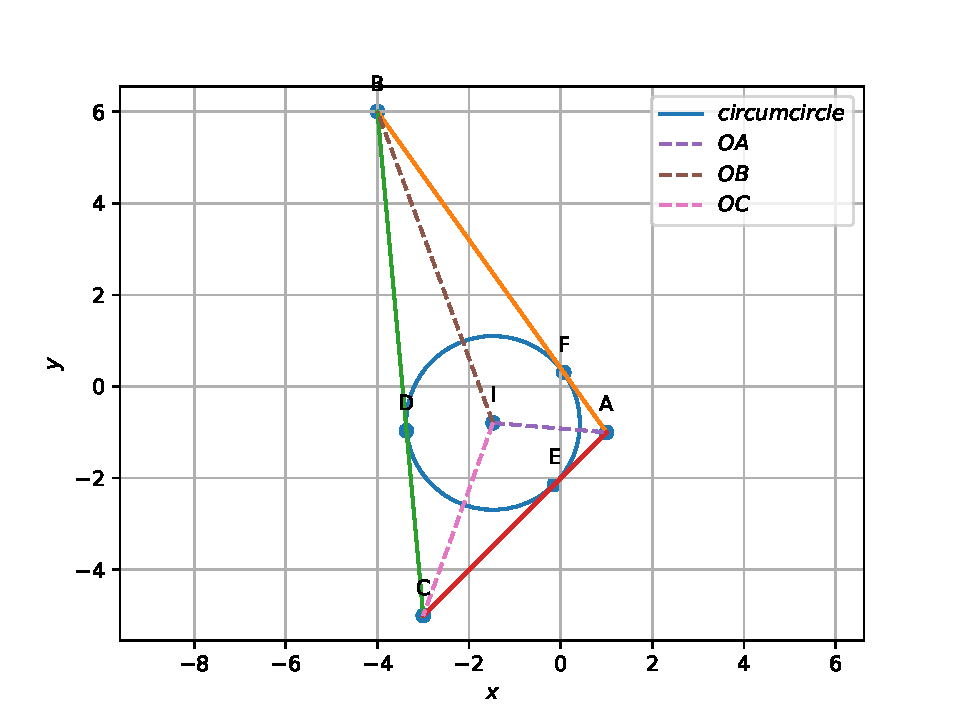
\includegraphics[width=\columnwidth]{figs/triangle/ang-bisect.pdf}
	\caption{Incircle of $\triangle ABC$}
	\label{fig:incircle}
\end{figure}
\iffalse
Considering
\begin{align}
	BC: \quad \vec{n} ^\top \vec{x} &= c, 
\end{align}
the distance from $\vec{I}$ to $BC$ is 
\begin{align}
\frac{\abs{\vec{n}^\top \vec{I} - c}}{\norm{\vec{n}}} 
\end{align}
\fi


	\item Using 
    \eqref{eq:app-angle2d}
verify that 
		\begin{align}
			\angle BAI = \angle CAI.
		\end{align}
		$AI$ is the bisector of $\angle A$.  
	\item Verify that $BI, CI$ are also the angle bisectors of $\triangle ABC$.
All codes for this section are available at
\begin{lstlisting}
	codes/triangle/ang-bisect.py
\end{lstlisting}

\end{enumerate}

\subsection{Eigenvalues and Eigenvectors}
\begin{enumerate}[label=\thesubsection.\arabic*.,ref=\thesubsection.\theenumi]
\item 
	 The equation of a circle is given by 
	\label{prop:circ-eq}
\begin{align}
	\norm{\vec{x}}^2 + 2 \vec{u}^{\top}\vec{x} + f = 0
	\label{eq:circ-eq}
\end{align}
for
		\begin{align}
			 \label{eq:conic_quad_form-params}
	 \vec{u}=-\vec{O}, f = \norm{\vec{O}}-r^2,
		\end{align}
		$\vec{O}$ being the incentre and $r$ the inradius.  
\item Compute 
\begin{align}
	\label{eq:incircle-disc-Sigma}
\vec{\Sigma} = 
\brak{\vec{V}\vec{h}+\vec{u}}
	  \brak{\vec{V}\vec{h}+\vec{u}}^{\top}
   -
	  {g}\brak{\vec{h}}\vec{V}
\end{align}
for $\vec{h}=\vec{A}$.
\item Find the roots of the equation
\begin{align}
	\mydet{\lambda \vec{I}-\vec{\Sigma}} = 0
\end{align}
These are known as the eigenvalues of $\vec{\Sigma}$.
\item Find $\vec{p}$  such that 
\begin{align}
	\vec{\Sigma}\vec{p}
	=\lambda\vec{p}
\end{align}
using row reduction.  These are known as the eigenvectors of $\Sigma$.
\item Define
    \begin{align}
      \label{eq:conic_parmas_eig_def-D}
      \vec{D} &= \myvec{\lambda_1 & 0\\ 0 & \lambda_2}, 
      \\
	    \vec{P} &= \myvec{\frac{\vec{p}_1}{\norm{\vec{p}_1}} & \frac{\vec{p}_2}{\norm{\vec{p}_2}}}
      \label{eq:eigevecP}
    \end{align}
    \item Verify that
  \begin{align}
\vec{P}^{\top}=\vec{P}^{-1}.
  \label{eq:orth-mat}
  \end{align}
  $\vec{P}$ is defined to be an orthogonal matrix.
\item Verify that
    \begin{align}
      \label{eq:conic_parmas_eig_def}
      \vec{P}^{\top}\vec{\Sigma}\vec{P} &= \vec{D},
    \end{align} 
		This is known as the spectral (eigenvalue ) decomposition of a symmetric matrix 

\item
	The direction vectors of the tangents from a point 
$\vec{h}$ to the circle in \eqref{eq:conic_quad_form} are given by  
\begin{align}
  \vec{m}&= \vec{P}\myvec{\sqrt{\abs{\lambda_2}} \\[2mm]  \pm \sqrt{\abs{\lambda_1}}}
	  \label{eq:h-tangents-cond-mPlam}
\end{align}
\item The points of contact of the pair 
of tangents 
to the circle in \eqref{eq:conic_quad_form} 
	from 
	a point $\vec{h}$ 
	are given by 
  \begin{align}
  \label{eq:line_dir_pt-lam}
	  \vec{x}  = \vec{h} + \mu \vec{m}
  \end{align}
  where 
  \begin{align}
  \label{eq:line_dir_pt-lam-mu}
	  \mu = -\frac{\vec{m}^{\top}\brak{\vec{V}\vec{h}+\vec{u}}}{\vec{m}^{\top}\vec{V}\vec{m} }
  \end{align}
	for $\vec{m}$ in 
	  \eqref{eq:h-tangents-cond-mPlam}.
  Compute the points of contact. You should get the same points that you obtained in the previous section. 

All codes for this section are available at
\begin{lstlisting}
	codes/triangle/tangpair.py
\end{lstlisting}
\end{enumerate}

\section{Matrices}
\numberwithin{equation}{section}
The matrix of the veritices of the triangle is defined as
		\begin{align}
			\vec{P} = \myvec{\vec{A} & \vec{B} &\vec{C}}
		\end{align}
		\subsection{Vectors}
\begin{enumerate}[label=\thesection.\arabic*.,ref=\thesubsection.\theenumi]
\numberwithin{equation}{enumi}
\item Obtain the direction matrix of the sides of $\triangle ABC$
	defined as 
		\begin{align}
		\vec{M} = 	\myvec{\vec{A}-\vec{B} & \vec{B}-\vec{C} & \vec{C}-\vec{A}}
		\end{align}
	\\
		\solution 

		\begin{align}
			\vec{M} &= \myvec{\vec{A}-\vec{B} & \vec{B}-\vec{C} & \vec{C}-\vec{A}}
			\\
			&= 
			\myvec{\vec{A} & \vec{B} &\vec{C}}
			\myvec{1 & 0 & -1 \\ -1 & 1 & 0 \\ 0 & -1 & 1}
		\end{align}
		where the second matrix above 
		is known as a {\em circulant} matrix.  Note that the 2nd and 3rd row of the above matrix are circular shifts of the 1st row.
	\item Obtain the normal matrix  of the sides of $\triangle ABC$
		\\
		\solution Considering the roation matrix
		\begin{align}
			\vec{R}  = \myvec{0 & -1 \\ 1 & 0},
		\end{align}
		the normal matrix is obtained as
		\begin{align}
			\vec{N} = \vec{R}\vec{M} 
		\end{align}

	\item Obtain $a, b, c$.
		\\
		\solution The sides vector is obtained as
		\begin{align}
			\vec{d} = \sqrt{\text{diag}(\vec{M}^{\top}\vec{M})}
		\end{align}
	\item Obtain the constant terms in the equations of the sides of the triangle. 
		\\
		\solution The constants for the lines can be expressed in vector form as
		\begin{align}
			\vec{c} = \text{diag}\cbrak{\brak{\vec{N}^{\top}\vec{P}}} 
		\end{align}
\end{enumerate}
		\subsection{Median}
\begin{enumerate}[label=\thesubsection.\arabic*.,ref=\thesubsection.\theenumi]
\numberwithin{equation}{enumi}
\item Obtain the mid point matrix for the sides of the triangle
	\\
		\solution
		\begin{align}
			\myvec{\vec{D} & \vec{E} &\vec{F}} &= \frac{1}{2}\myvec{\vec{A} & \vec{B} &\vec{C}}
			\myvec{0 & 1 & 1 \\ 1 & 0 & 1 \\ 1 & 1 & 0}
		\end{align}
	\item Obtain the median direction matrix.
\\
\solution The median direction matrix is given by 
		\begin{align}
			\vec{M}_1 &= \myvec{\vec{A}-\vec{D} & \vec{B}-\vec{E} & \vec{C}-\vec{F}}
			\\
			&= 
			  \myvec{
				  \vec{A}-\frac{\vec{B}+\vec{C}}{2} &
			  \vec{B}-\frac{\vec{C}+\vec{A}}{2} &
			  \vec{C}-\frac{\vec{A}+\vec{B}}{2}} 
			  \\
			  &= \myvec{\vec{A} & \vec{B} &\vec{C}}
			  \myvec{
				  1 & -\frac{1}{2} & -\frac{1}{2}
				  \\
				  -\frac{1}{2} & 1 & -\frac{1}{2}
				  \\
				  -\frac{1}{2} & -\frac{1}{2} & 1
				  }
		\end{align}
	\item Obtain the median normal matrix.
	\item Obtian the median equation constants.
	\item Obtain the centroid by finding the intersection of the medians.

\end{enumerate}
		\subsection{Altitude}
\begin{enumerate}[label=\thesubsection.\arabic*.,ref=\thesubsection.\theenumi]
\numberwithin{equation}{enumi}
\item Find the normal matrix for the altitudes
	\\
		\solution  The desired matrix is 
\begin{align}
	\vec{M}_2 &= 	\myvec{\vec{B}-\vec{C} & \vec{C}-\vec{A} & \vec{A}-\vec{B} }
	\\
	&= 
	\myvec{\vec{A} & \vec{B} &\vec{C}}
			\myvec{ 0 & -1 & 1 \\ 1 & 0 & -1 \\ -1 & 1 & 0}
		\end{align}

	\item Find the constants vector for the altitudes.
		\\
		\solution The desired vector is 
		\begin{align}
			\vec{c}_2 = \text{diag}\cbrak{\brak{\vec{M}^{\top}\vec{P}}} 
		\end{align}
\end{enumerate}
		\subsection{Perpendicular Bisector}
\begin{enumerate}[label=\thesubsection.\arabic*.,ref=\thesubsection.\theenumi]
\numberwithin{equation}{enumi}
\item Find the normal matrix for the perpendicular bisectors
	\\
	\solution The normal matrix is $\vec{M}_2$
\item Find the constants vector for the perpendicular bisectors.
		\\
		\solution The desired vector is 
		\begin{align}
			\vec{c}_3 = \text{diag}\cbrak{\vec{M}_2^{\top}\myvec{\vec{D} & \vec{E} &\vec{F}}}
		\end{align}

\end{enumerate}
		\subsection{Angle Bisector}
\begin{enumerate}[label=\thesubsection.\arabic*.,ref=\thesubsection.\theenumi]
\numberwithin{equation}{enumi}
\item Find the points of contact.
	\\
		\solution The points of contact are given by 
		\begin{align}
			\myvec{			
						\frac{m\vec{C}+n\vec{B}}{m+n}
			&
			\frac{n\vec{A}+p\vec{C}}{n+p}
			&
						\frac{p\vec{B}+m\vec{A}}{p+m}
			}
			= 	\myvec{\vec{A} & \vec{B} &\vec{C}}
			\myvec{
				0 &			\frac{n}{b} & \frac{m}{c}  
				\\
			 \frac{n}{a}& 0 & \frac{p}{c} 
				\\
			\frac{m}{a}	&		\frac{p}{b} & 0  
			}
		\end{align}
All codes for this section are available at
\begin{lstlisting}
	codes/triangle/mat-alg.py
\end{lstlisting}
\end{enumerate}


%\section{Quadrilateral}
%\renewcommand{\theequation}{\theenumi}
\begin{enumerate}[label=\arabic*.,ref=\thesubsection.\theenumi]
\numberwithin{equation}{enumi}
	%
%
%
%
%
\item Parallelograms on the same base (or equal bases) and between the same parallels are equal in area.
\item If a parallelogram and a triangle are on the same base and between the same parallels, then area of the triangle is half the area of the parallelogram.
%
\item  The quadrilateral formed by joining the mid-points of the sides of a quadrilateral, in order, is a parallelogram.
%
%
\item Two parallel lines l and m are intersected by a transversal p. Show that the quadrilateral formed by the bisectors of interior angles is a rectangle.
%
\item Show that the bisectors of angles of a parallelogram form a rectangle.
%
%
\item $ABCD$ is a parallelogram in which $P$ and $Q$ are mid-points of opposite sides $AB$ and $CD$. If $AQ$ intersects $DP$ at $S$ and $BQ$ intersects $CP$ at $R$, show that: 
%
\begin{enumerate}
\item  $APCQ$ is a parallelogram. 
\item $DPBQ$ is a parallelogram. 
\item $PSQR$ is a parallelogram.
\end{enumerate}
%
\item $l, m$ and $n$ are three parallel lines intersected by transversals $p$ and $q$ such that $l, m$ and $n$ cut off equal intercepts $AB$ and $BC$ on $p$ . Show that $l, m$ and $n$ cut off equal intercepts $DE$ and $EF$ on $q$ also.
%
\item Parallelograms on the same base (or equal bases) and between the same parallels are equal in area.
\item Area of a parallelogram is the product of its base and the corresponding altitude. 
\item Parallelograms on the same base (or equal bases) and having equal areas lie between the same parallels.
\item If a parallelogram and a triangle are on the same base and between the same parallels, then area of the triangle is half the area of the parallelogram.
\item In parallelogram $ABCD$, two points $P$ and $Q$ are taken on diagonal $BD$ such that $DP = BQ$. show that \begin{enumerate}
 \item  $\triangle  APD  \cong   \triangle  CQB$ 
\item $AP = CQ$ \item  $\triangle  AQB  \cong   \triangle  CPD$ 
\item $AQ = CP$ 
\item $APCQ$ is a parallelogram
\end{enumerate}
\item $ABCD$ is a parallelogram and $AP$ and $CQ$ are perpendiculars from vertices $A$ and $C$ on diagonal $BD$ . Show that 
\begin{enumerate} 
\item  $\triangle  APB  \cong   \triangle  CQD $ 
\item $AP = CQ$
\end{enumerate}
%
\item In  $\triangle  ABC$ and  $\triangle  DEF, AB = DE, AB  \parallel  DE, BC = EF$ and $BC  \parallel  EF$. Vertices $A, B$ and $C$ are joined to vertices $D, E$ and $F$ respectively. Show that 
\begin{enumerate}
\item quadrilateral $ABED$ is a parallelogram 
\item quadrilateral $BEFC$ is a parallelogram 
\item $AD  \parallel  CF$ and $AD = CF$ 
\item quadrilateral $ACFD$ is a parallelogram 
\item $AC$ = $DF$ 
\item  $\triangle  ABC  \cong   \triangle  DEF$.
%
\end{enumerate}

\item $ABCD$ is a trapezium in which $AB$  $\parallel$  $CD$ and $AD = BC$. Show that 
\begin{enumerate} 
\item$\angle A$ =  $\angle B$  
\item  $\angle C  =  \angle D$  \item  $\triangle  ABC  \cong   \triangle  BAD$ 
\item diagonal $AC$ = diagonal $BD$ 
\end{enumerate}
%
\item $ABCD$ is a quadrilateral in which $P, Q, R$ and $S$ are mid-points of the sides $AB, BC, CD$ and $DA$ $AC$ is a diagonal. Show that 
\begin{enumerate} 
\item $SR$  $\parallel$  $AC$ and $SR =\frac{1}{ 2}AC$
\item $PQ = SR$ 
\item  $PQRS$  is a parallelogram.
\end{enumerate}
%
\item $ABCD$ is a rhombus and  $P, Q, R$ and $S$  are the mid-points of the sides  $AB, BC, CD$ and $DA$ respectively. Show that the quadrilateral  $PQRS$  is a rectangle.
\item $ABCD$ is a rectangle and  $P, Q, R$ and $S$  are mid-points of the sides  $AB, BC, CD$ and $DA$ respectively. Show that the quadrilateral  $PQRS$  is a rhombus.
\item $ABCD$ is a trapezium in which $AB  \parallel  DC, BD$ is a diagonal and $E$ is the mid-point of $AD$. A line is drawn through $E$ $\parallel$  $AB$ intersecting $BC$ at $F$. Show that $F$ is the mid-point of $BC$.
\item In a parallelogram $ABCD$, $E$ and $F$ are the mid-points of sides $AB$ and $CD$ respectively . Show that the line segments $AF$ and $EC$ trisect the diagonal $BD$.
\item Show that the line segments joining the mid-points of the opposite sides of a quadrilateral bisect each other.
\item $ABCD$ is a parallelogram in which $P$ and $Q$ are mid-points of opposite sides $AB$ and $CD$. If $AQ$ intersects $DP$ at $S$ and $BQ$ intersects $CP$ at $R$, show that: 
%
\begin{enumerate}
\item  $APCQ$ is a parallelogram. 
\item $DPBQ$ is a parallelogram. 
\item $PSQR$ is a parallelogram.
\end{enumerate}
%
\item $l, m$ and $n$ are three parallel lines intersected by transversals $p$ and $q$ such that $l, m$ and $n$ cut off equal intercepts $AB$ and $BC$ on $p$ . Show that $l, m$ and $n$ cut off equal intercepts $DE$ and $EF$ on $q$ also.
%
\item Diagonal $AC$ of a parallelogram $ABCD$ bisects $\angle A$ . show that 
\begin{enumerate}
\item it bisects  $\angle C$  also, 
\item $ABCD$ is a rhombus.
\end{enumerate}
%
\item $ABCD$ is a rhombus. Show that diagonal $AC$ bisects $\angle A$ as well as  $\angle C$  and diagonal $BD$ bisects  $\angle B$  as well as  $\angle D$ .
\item $ABCD$ is a rectangle in which diagonal $AC$ bisects $\angle A$ as well as  $\angle C$ . Show that 
\begin{enumerate}
\item $ABCD$ is a square 
\item diagonal $BD$ bisects  $\angle B$  as well as  $\angle D$ .
%
\end{enumerate}

\item If $E,F,G$ and $H$ are respectively the mid-points of the sides of a parallelogram $ABCD$, show that
\begin{align}
ar \brak{EFGH} =
\frac{1}{ 2}
ar \brak{ABCD} .
\end{align}
%
\item $P$ and $Q$ are any two points lying on the sides $DC$ and $AD$ respectively of a parallelogram $ABCD$. Show that $ar (APB) = ar (BQC)$.
%
\item P is a point in the interior of a parallelogram $ABCD$. Show that
\begin{enumerate}
\item $ar (APB) + ar (PCD) = \frac{1}{ 2}ar (ABCD)$
\item $ar (APD) + ar (PBC) = ar (APB) + ar (PCD)$
\end{enumerate}
%
\item $PQRS$ and $ABRS$ are parallelograms and $X$ is any point on side $BR$. show that 
\begin{enumerate} 
\item $ar (PQRS) = ar (ABRS)$
\item $ar (AX S) = \frac{1}{ 2} ar (PQRS)$
\end{enumerate}
%
\item A farmer was having a field in the form of a parallelogram $PQRS$. She took any point $A$ on $RS$ and joined it to points $P$ and $Q$. In how many parts the fields is divided? What are the shapes of these parts? The farmer wants to sow wheat and pulses in equal portions of the field separately. How should she do it?
%
\item $ABCD$ is a quadrilateral and $BE  \parallel  AC$ and also $BE$ meets $DC$ produced at $E$. Show that area of $ \triangle  ADE$ is equal to the area of the quadrilateral $ABCD$.
%
\item $E$ is any point on median $AD$ of a  $\triangle  ABC$. Show that $ar (ABE) = ar (ACE)$.
\item  In a $\triangle ABC, E$ is the mid-point of median $AD$. Show that $ar (BED) = \frac{1}{ 4}ar(ABC)$ .
\item  Show that the diagonals of a parallelogram divide it into four triangles of equal area.
\item   $ABC$ and $ABD$ are two triangles on the same base $AB$. If line- segment $CD$ is bisected by $AB$ at $O$, show that $ar(ABC) = ar (ABD)$.
%
\item $D$, $E$ and $F$ are respectively the mid-points of the sides $BC, CA$ and $AB$ of a $ \triangle  ABC$. show that 
\begin{enumerate}
\item $BDEF$ is a parallelogram. 
\item $ar (BDEF) =
\frac{1}{ 2}
ar (ABC)$
\end{enumerate}
%
\item   Diagonals $AC$ and $BD$ of quadrilateral $ABCD$ intersect at $O$ such that $OB = OD$. If $AB = CD$, then show that 
\begin{enumerate}
\item $ar (DOC) = ar (AOB)$
 \item $ar (DCB) = ar (ACB)$
\item $ar (DEF) =
\frac{1}{ 4}
ar (ABC)$ 
\end{enumerate}
\item $D$ and $E$ are points on sides $AB$ and $AC$ respectively of $ \triangle  ABC$ such that $ar (DBC) = ar (EBC)$. Prove that $DE  \parallel  BC$.
\item $XY$ is a line parallel to side $BC$ of a $\triangle ABC$. If $BE  \parallel  AC$ and $CF  \parallel  AB$ meet $XY$ at $E$ and $F$ respectively, show that
$ar (ABE) = ar (ACF)$.
\item The side $AB$ of a parallelogram $ABCD$ is produced to any point $P$. A line through $A$ and parallel to $CP$ meets $CB$ produced at $Q$ and then parallelogram $PBQR$ is completed. Show that $ar ($ABCD$) = ar (PBQR)$. \item Diagonals $AC$ and $BD$ of a trapezium $ABCD$ with $AB  \parallel  DC$ intersect each other at $O$. Prove that $ar (AOD) = ar (BOC)$.
\item  $ABCDE$ is a pentagon. A line through $B$ parallel to $AC$ meets $DC$ produced at $F$. Show that 
\begin{enumerate}
\item $ar (ACB) = ar (ACF)$
 \item $ar (AEDF) = ar (ABCDE)$
. 
\end{enumerate}
\item A villager Itwaari has a plot of land of the shape of a quadrilateral. The Gram Panchayat of the village decided to take over some portion of his plot from one of the corners to construct a Health Centre. Itwaari agrees to the above proposal with the condition that he should be given equal amount of land in lieu of his land adjoining his plot so as to form a triangular plot. Explain how this proposal will be implemented.
\item $ABCD$ is a trapezium with $AB  \parallel  DC$. A line parallel to $AC$ intersects $AB$ at $X$ and $BC$ at $Y$. Prove that $ar (ADX) = ar (ACY)$.
\item  $AP  \parallel  BQ  \parallel  CR$. Prove that $ar (AQC) = ar (PBR)$.
\item Diagonals $AC$ and $BD$ of a quadrilateral $ABCD$ intersect at $O$ in such a way that $ar (AOD) = ar (BOC)$. Prove that $ABCD$ is a trapezium.
\item  $AB \parallel DC \parallel RP$.  $ar (DRC) = ar (DPC)$ and $ar (BDP) = ar (ARC)$. Show that both the quadrilaterals $ABCD$ and $DCPR$ are trapeziums.

\item Parallelogram $ABCD$ and rectangle $ABEF$ are on the same base $AB$ and have equal areas. Show that the perimeter of the parallelogram is greater than that of the rectangle.
\item  In $\triangle ABC$,  $D$ and $E$ are two points on $BC$ such that $BD = DE = EC$. Show that $ar (ABD) = ar (ADE) = ar (AEC)$.
\item $ABCD, DCFE$ and $ABFE$ are parallelograms. Show that ar$ (ADE) = ar (BCF)$.
\item  $ABCD$ is a parallelogram and $BC$ is produced to a point $Q$ such that $AD = CQ$. If $AQ$ intersect $DC$ at $P$, show that $ar (BPC) = ar (DPQ)$.
$ABC$ and $BDE$ are two equilateral triangles such that $D$ is the mid-point of $BC$. If $AE$ intersects $BC$ at$ F$, show that 
\begin{enumerate}
\item $ar (BDE) = \frac{1}{ 4} ar (ABC)$
\item $ar (BDE) = \frac{1}{ 2} ar (BAE)$
\item $ar (ABC) = 2 ar (BEC)$
 \item $ar (BFE) = ar (AFD)$ 
\item $ar (BFE) = 2 ar (FED)$
\item $ar (FED) =
\frac{1}{ 8}
ar (AFC)$
\end{enumerate}
\item Diagonals $AC$ and $BD$ of a quadrilateral $ABCD$ intersect each other at $P$. Show that $ar (APB)  \times  ar (CPD) = ar (APD)  \times  ar (BPC)$.
\item  $P$ and $Q$ are respectively the mid-points of sides AB and BC of a $\triangle ABC$ and $R$ is the mid-point of $AP$, show that 
\begin{enumerate}
\item $ar (PRQ) = \frac{1 }{2}ar (ARC) $
\item $ar (PBQ) = ar (ARC)$
\item $ar (RQC) =
\frac{3}{ 8}
ar (ABC)$
\end{enumerate}
%
\item $ABC$ is a right triangle right angled at $A$. $BCED$, $ACFG$ and $ABMN$ are
squares on the sides $BC, CA$ and $AB$ respectively. Line segment $AX \perp  DE$ meets $BC$ at $Y$. Show that 
\begin{enumerate}
\item $ \triangle  MBC \cong  \triangle  ABD$
\item $ar (BYXD) = ar (ABMN)$ \item $ar (CYXE) = 2 ar (FCB)$
\item $ar (BYXD) = 2 ar (MBC)$ 
\item $ \triangle  FCB \cong  \triangle  ACE$
\item $ar (CYXE) = ar (ACFG)$
\item  $ar (BCED) = ar (ABMN) + ar (ACFG)$
\end{enumerate}
\item $L$ is a point on the diagonal $AC$ of quadrilateral $ABCD$.  If LM || CB and LN || CD, prove that $\frac{AM}{AB}=\frac{ AN}{  AD}$
\item The angles of quadrilateral are in the ratio 3 : 5 : 9 : 13. Find all the angles of the quadrilateral.
\\
\solution
%\renewcommand{\theequation}{\theenumi}
%\begin{enumerate}[label=\arabic*.,ref=\thesubsection.\theenumi]
%\numberwithin{equation}{enumi}
%
 Let the measure of angles $\phase{A},\phase{B},\phase{C},\phase{D} $ of a quadrilateral are 3x, 5x, 9x and 13x respectively, where x is a real number.
\\
Using angle sum property, the sum of interior angles of a quadrilateral is 360 degree.
\begin{align}
3x+5x+9x+13x=360\degree
\\
30x=360\degree
\\
x=12\degree
\end{align}
 From the above calculations, 
 \begin{align}
 \phase{A}=3x=3(12)=36\degree
 \\
 \phase{B}=5x=5(12)=60\degree
 \\
 \phase{C}=9x=9(12)=108\degree
 \\
 \phase{D}=13x=13(12)=156\degree
 \end{align}


\end{enumerate}


\appendices
\section{Tangents to a Circle}
\numberwithin{equation}{section}
The equation of the {\em incircle} is given by 
		\begin{align}
			\label{eq:incircle}
			\norm{\vec{x}-\vec{O}}^2 = r^2
		\end{align}
		which can be expressed as 
			 \eqref{eq:conic_quad_form}
			 using 
			 \eqref{eq:conic_quad_form-params}.
	In \figref{fig:incircle}, 
Let 
  \eqref{eq:line_dir_pt-lam}
  be the equation of $AB$.  Then, the intersection of 
  \eqref{eq:line_dir_pt-lam}
  and 
			 \eqref{eq:conic_quad_form}
			 can be expressed as 
\begin{align}
\brak{\vec{h} + \mu{\vec{m}}}^{\top}
\vec{V}
\brak{\vec{h} + \mu{\vec{m}}}
			+2\vec{u}^{\top}\brak{\vec{h} + \mu{\vec{m}}}+f &= 0
			\\
\implies \mu^2\vec{m}^{\top} \vec{V}\vec{m} + 2\mu \vec{m}^{\top}\brak{\vec{V}\vec{h}+\vec{u}}+g\brak{\vec{h}} &= 0 
	\label{eq:incircle-quad}
\end{align}
For 	\eqref{eq:incircle-quad} to have exactly one root, the discriminant
\begin{align}
 \cbrak{\vec{m}^{\top}\brak{\vec{V}\vec{h}+\vec{u}}}^2 -g\brak{\vec{h}}\vec{m}^{\top} \vec{V}\vec{m}  &= 0 
	\label{eq:incircle-disc}
\end{align}
and 
  \eqref{eq:line_dir_pt-lam-mu}
  is obtained.
	\eqref{eq:incircle-disc}
	can be expressed as
\begin{align}
\vec{m}^{\top}\brak{\vec{V}\vec{h}+\vec{u}}^{\top}\brak{\vec{V}\vec{h}+\vec{u}}\vec{m}-g\brak{\vec{h}}\vec{m}^{\top} \vec{V}\vec{m}  &= 0 
\\
\implies \vec{m}^{\top}\vec{\Sigma}\vec{m} &= 0
	\label{eq:incircle-disc-Sigma-new}
\end{align}
for $\vec{\Sigma}$ defined in 
	\eqref{eq:incircle-disc-Sigma-new}.
      Substituting \eqref{eq:conic_parmas_eig_def}
	in \eqref{eq:incircle-disc-Sigma-new},
\begin{align}
\vec{m}^{\top}\vec{P}\vec{D}\vec{P}^{\top}\vec{m} &= 0
\\
\implies 
\vec{v}^{\top}\vec{D}\vec{v} &= 0
	\label{eq:incircle-disc-v}
\end{align}
where 
\begin{align}
	\label{eq:incircle-disc-v-lam-P}
\vec{v} = \vec{P}^{\top}\vec{m}
\end{align}
	\eqref{eq:incircle-disc-v}
	can be expressed as 
\begin{align}
\lambda_1 v_1^2
-\lambda_2 v_2^2 &= 0
\\
\implies \vec{v} = \myvec{\sqrt{\abs{\lambda_2}} \\[2mm]  \pm \sqrt{\abs{\lambda_1}}}
	\label{eq:incircle-disc-v-lam}
\end{align}
after some algebra.
From 
	\eqref{eq:incircle-disc-v-lam}
	and
	\eqref{eq:incircle-disc-v-lam-P}
	we obtain 
	  \eqref{eq:h-tangents-cond-mPlam}.



\iffalse
\latexprintindex
\fi

\end{document}

